% =============================================================================
% K=5 VARIANT of the troposwhere manuscript (duplicated from paper/manuscript/).
% Mechanical substitutions applied: K=7 -> K=5; "seven" -> "five" in
% state-count language; pi vector, lambda_2, and v_2 swapped to K=5 numbers
% (from paper/reports/cluster_comparison/numbers.json).
% Body prose and figures fully migrated to K=5 (all six critical figures
% regenerated via paper_5clusters/notebooks/figures_paper_5c.py).
% Remaining TODOs live in supplementary.tex (SI figures + sensitivity
% section) and are tracked in ../TODO_5c.md.
% =============================================================================
\documentclass[11pt]{article}

% ── Layout & typography ─────────────────────────────────────────────────
\usepackage[margin=2.2cm]{geometry}              % tighter margins (default ~3.5cm)
\usepackage[T1]{fontenc}
\usepackage[utf8]{inputenc}
\usepackage{lmodern}                              % modern Computer Modern
\usepackage{microtype}                            % subtle typographic improvements
\usepackage{setspace}\setstretch{1.15}            % a touch more line spacing
\usepackage{parskip}                              % blank line between paragraphs, no indent
\usepackage{lineno}\linenumbers                   % line numbers (for reviewers)
\usepackage[font=small,labelfont=bf]{caption}     % small captions with bold "Figure N."
\setlength{\emergencystretch}{2em}                % reduce Overfull \hbox warnings

% ── Math, figures, references ──────────────────────────────────────────
\usepackage{amsmath}
\usepackage{amssymb}
\usepackage{graphicx}
\usepackage{comment}
\usepackage{url}
\usepackage{xcolor}                               % needed for blue!50!black, teal!60!black, etc.
\usepackage[colorlinks=true, allcolors=blue!50!black, citecolor=teal!60!black]{hyperref}
\usepackage{xr-hyper}                             % cross-document refs (e.g. SI labels)
\externaldocument{supplementary}                  % reads supplementary.aux if present
\usepackage[
    backend=biber,
    style=authoryear,
    sorting=nyt,
    natbib=true
]{biblatex}
\addbibresource{biblio.bib}

% ── Optional draft watermark ───────────────────────────────────────────
%\usepackage{draftwatermark}
%\SetWatermarkText{DRAFT}
%\SetWatermarkScale{2.5}

\graphicspath{{./}{figures/}{SI_figures/}{img/}}

% \title{Convective Organization as Markov Trajectories in Latent Space}
\title{A temporally-constrained latent space \\ reveals the stochastic dynamics of convective organization}
\author{Sophie Abramian, Olivier Pauluis, Pierre Gentine}
\date{June 2026}

\begin{document}

\maketitle


\section*{Abstract}
% Previous abstract (long form, preserved for reference):
% Convective storms are stochastic, high-dimensional systems whose evolution resists compact description. Here we focus on their internal variability---the diversity of storm evolution that emerges under a fixed large-scale environment rather than from changes in the forcing itself. We introduce a framework that treats convective organization dynamically: an encoder maps isentropic mass-flux profiles into a low-dimensional latent space, the latent space is partitioned into discrete convective states, and transitions between states are modelled as a Markov chain. Applied to cloud-resolving simulations of squall lines under fixed vertical wind shear, the model identifies eight latent dimensions and five states recovering the canonical phases of the convective life cycle. The learned dynamics expose two pathways: a direct route into sustained deep convection and a slower route through weakly organized phases. Departures from strict Markovianity in the organized regime expose the role of internal feedbacks---particularly cold-pool dynamics---as sources of effective memory; conditioning on cold-pool intensity at the starting time partly restores Markovian behaviour, suggesting that explicitly embedding such internal processes improves model fidelity. The results indicate that convective diversity arises from the range of dynamical trajectories supported by the environment rather than from distinct states alone, and offer a learned, stochastic alternative to prescribed multi-cloud parameterizations.
Atmospheric convection is a stochastic, high-dimensional process: under identical large-scale forcing, storms evolve along widely different trajectories, and capturing this internal variability remains a central challenge for climate models. Here we introduce an unsupervised framework that learns a compact, dynamically meaningful representation of convective evolution. An encoder maps isentropic vertical mass-flux fields, obtained from cloud-resolving simulations of squall lines, into a low-dimensional latent space. Two constraints shape this space: a reconstruction loss that preserves its physical content, and a linear stochastic operator trained to predict the next time step. This temporal constraint reshapes the latent space into a physically structured representation, organized along emergent and interpretable axes of intensity and organization, in which five canonical convective regimes---suppressed, shallow congestus, active-unorganized, mesoscale stratiform, and organized deep convection---are recovered without human supervision. The associated Markov transition matrix exposes two coupled dynamical regimes---organized and unorganized convection---separated by a suppressed background, with a slow eigenmode alternating between them. A Markovianity assessment further reveals residual memory in the long-lived regimes; conditioning on cold-pool intensity at the starting time closes about a third of this gap, identifying cold pools as a measurable carrier of effective memory. The framework offers a learned, stochastic alternative to prescribed multi-cloud parameterizations and a route to embedding internal convective variability into climate models.

\section{Introduction}

Convective storms are high-dimensional dynamical systems whose collective behavior controls vertical transports of mass, energy and moisture, and whose representation in coarse-grained climate models remains a persistent challenge---particularly under warming \citep{yang2023impact, bolot2025no, prein2022towards, chakraborty2023overview}. A central difficulty is that the convective response to a \emph{fixed} large-scale forcing is not a single outcome but a broad distribution of storm evolutions \citep{abramian2025key, feng2025mesoscale, hu2020observed, fiolleau2024database}: an \emph{internal} variability intrinsic to the convection itself, not inherited from changes in the environment. Capturing it requires a reduced description that is both low-dimensional---so it can be embedded in a climate model---and faithful to the underlying dynamics.

Existing reductions---stochastic multi-cloud models \citep{khouider2006multicloud, majda2008stochastic, khouider2010stochastic}---prescribe a small set of cloud types \emph{a priori} and impose Markov transitions over them. This captures storm-population dynamics but cannot resolve the diversity of vertical mass-flux profiles that govern extreme precipitation \citep{MullerYukari19, singh2012upward, abramian2023extreme, wang2022convective, li2025bimodal}. Koopman operator theory \citep{koopman1931hamiltonian, brunton2021modern} offers a principled alternative: one constructs nonlinear observables of the physical state in which the evolution becomes exactly linear. This linearization comes at a cost---the full Koopman operator is infinite-dimensional, and physically meaningful observables are not known \emph{a priori}. Encoder--decoder architectures \citep{lusch2018deep, nathaniel2026generative} resolve both: they learn finite-dimensional observables and their linear dynamics from data.

We build on this framework and depart from existing Koopman autoencoders in two ways. We cast the convective flow in isentropic coordinates \citep{pauluis2013isentropic}---a thermodynamically consistent substrate that preserves energetic structure and filters reversible adiabatic motions. And rather than enforcing \emph{deterministic} linear dynamics on the learned observables, we \emph{partition} the latent space into a finite set of discrete states through joint clustering \citep{kaiser2014cluster, souza2024representing} and model transitions between them \emph{probabilistically}. The reduced model that emerges is a Markov chain on data-discovered states---finite-dimensional, linear, memoryless by construction, stochastic by design, and shaped by the very dynamics it must represent.

Applied to squall lines simulated with the System for Atmospheric Modeling (SAM) under fixed vertical wind shear, this construction addresses three questions:
\begin{enumerate}
\item[(i)] What are the dominant convective mass-flux states accessible under a given forcing, here characterized by vertical wind shear?
\item[(ii)] Can transitions between these states be approximated by a Markov chain, and do the pathways differ between weakly and strongly organized convection?
\item[(iii)] To what extent is convective variability memoryless, and where do internal feedbacks---cold-pool dynamics in particular---introduce effective memory?
\end{enumerate}

The chain recovers, without supervision, five physically interpretable regimes spanning suppressed convection, shallow congestus, active unorganized, mesoscale stratiform, and moist deep-organized convection, modulated by a slow ($\sim$3\,h) eigenmode that alternates the chain between organized and unorganized periods. Two regimes---the moist deep-organized and the active-unorganized---decay more slowly than their own Markov prediction; this residual non-Markovianity quantifies the memory carried by internal feedbacks the partition does not see. Conditioning on cold-pool intensity at the starting time closes $\sim$30\% of the gap for the deep-organized regime, identifying cold pools as a measurable carrier of part of that memory.

Section~\ref{sec:methods} describes the methodology, Section~\ref{sec:results} develops the regimes and the Markovianity diagnostic, and Section~\ref{sec:discussion} discusses implications.

\section{Methods}\label{sec:methods}

\subsection{Idealized cloud-resolving simulations}

To examine the response of convection to fixed vertical wind shear, we perform idealized cloud-resolving simulations using the System for Atmospheric Modeling (SAM) \cite{khairoutdinov2003}. Following \cite{muller2013impact}, a low-level shear profile is imposed (see also \cite{rotunno1988theory, houze1977structure, robe2001effect}). The wind profile is linear, with a basal velocity of $8.5\,\mathrm{m\,s^{-1}}$ and a shear depth of $1\,\mathrm{km}$. This value is deliberately suboptimal relative to the shear magnitude ($\sim10\,\mathrm{m\,s^{-1}}$) that maximizes convective organization, in order to enhance sensitivity to internal variability (\cite{abramian2022shear}). In this regime, the balance between shear and cold-pool dynamics is more unstable, and variations in cold-pool properties exert a substantial control on convective development.

The model domain spans $128\,\mathrm{km} \times 128\,\mathrm{km}$ horizontally and extends from the surface to $17\,\mathrm{km}$ in the vertical, with enhanced resolution in the boundary layer. A sponge layer is applied near the model top to absorb upward-propagating gravity waves. Microphysical processes are represented using a single-moment scheme. The simulation is first integrated for 30 days to reach radiative--convective equilibrium and then continued for an additional 27 days for analysis. Model output is saved at 2-min intervals, yielding approximately $2\times10^{4}$ time steps, and includes both two- and three-dimensional fields. Under the imposed shear, convection self-organizes into squall-line structures oriented perpendicular to the shear direction, as illustrated in Fig.~\ref{fig:simu_isentrop}. The system alternates between quiescent phases and episodes of strong organization. Despite identical large-scale forcing, pronounced variability emerges in the structure, intensity, and persistence of the organized convective systems.

\subsection{Isentropic mass flux analysis and preprocessing}

Vertical transport associated with moist convection is inherently three-dimensional, intermittent, and multiscale. When diagnosed directly in physical space, the vertical mass flux reflects the superposition of contributions from convective updrafts and downdrafts, gravity waves, compensating subsidence, and turbulent fluctuations. This combination produces a noisy, high-dimensional field, making it difficult to isolate the collective transport by convection or to compare it consistently across realizations.

A physically grounded reduction of this complexity is provided by isentropic analysis \cite{pauluis2013isentropic}. Rather than organizing vertical motion by spatial location, this approach conditions transport on thermodynamic variables that are approximately conserved following moist adiabatic motion \cite{chen2022crucial}. In the moist atmosphere, we approximate isentropic surfaces using the moist static energy variable $h$. Projecting the vertical mass flux onto $h$ therefore reorganizes transport according to the energetic content of moving air parcels, rather than their instantaneous spatial position.

We define the moist static energy and the associated vertical isentropic mass flux as
\begin{align}
    h(x,y,z,t) & = c_p\, T(x,y,z,t)+ g\, z + L_v\, q_v(x,y,z,t),\\ 
    M(h,z,t) &= \int_{0}^{N_x}\int_{0}^{N_y} \rho(z,t)\,w(x,y,z,t)\,
    \delta\!\left(\hat{h}(x,y,z,t)-h\right)\,dx\,dy,
\end{align}
where $h(x,y,z,t)$ denotes the moist static energy, $c_p$ is the specific heat capacity of air at constant pressure, $T(x,y,z,t)$ is the absolute temperature, $g$ is the gravitational acceleration, $z$ is height, $L_v$ is the latent heat of vaporization, and $q_v(x,y,z,t)$ is the water vapor mixing ratio. The quantity $M(h,z,t)$ denotes the vertical isentropic mass flux, defined as the horizontal integral of the vertical mass flux $\rho(z,t)\,w(x,y,z,t)$ projected onto moist static energy levels using the Dirac delta function $\delta(\cdot)$. Here $\rho(z,t)$ is the air density, $w(x,y,z,t)$ is the vertical velocity, $\hat{h}(x,y,z,t)$ denotes the local moist static energy field, and $N_x$ and $N_y$ are the horizontal domain dimensions.

This thermodynamic conditioning performs two key functions. First, it reduces dimensionality by collapsing horizontal spatial variability into a compact $(h,z)$ phase space that retains the dominant structure of vertical transport. Second, it separates dynamically distinct processes that overlap in physical space but differ in thermodynamic character. Convective updrafts preferentially transport high $h$ air upward, entraining and evaporatively cooled downdrafts populate lower $h$ levels, while gravity-wave motions—characterized by weak net thermodynamic transport—are confined to low $h$ regions of the phase space\citep{chen2018atmospheric, chen2020significant}.

Within this isentropic representation, vertical transport organizes into coherent and interpretable patterns \citep{mrowiec2016isentropic}. Sustained positive mass flux at high $h$ extending through the troposphere is characteristic of deep convection, while shallow convection appears as weaker transport rapidly diluted by entrainment. Precipitating systems exhibit enhanced downdraft signatures and broadened $h$ distributions, and cold-pool dynamics manifest as near-surface, low-$h$ mass flux associated with evaporative cooling.

\begin{figure}
    \centering
    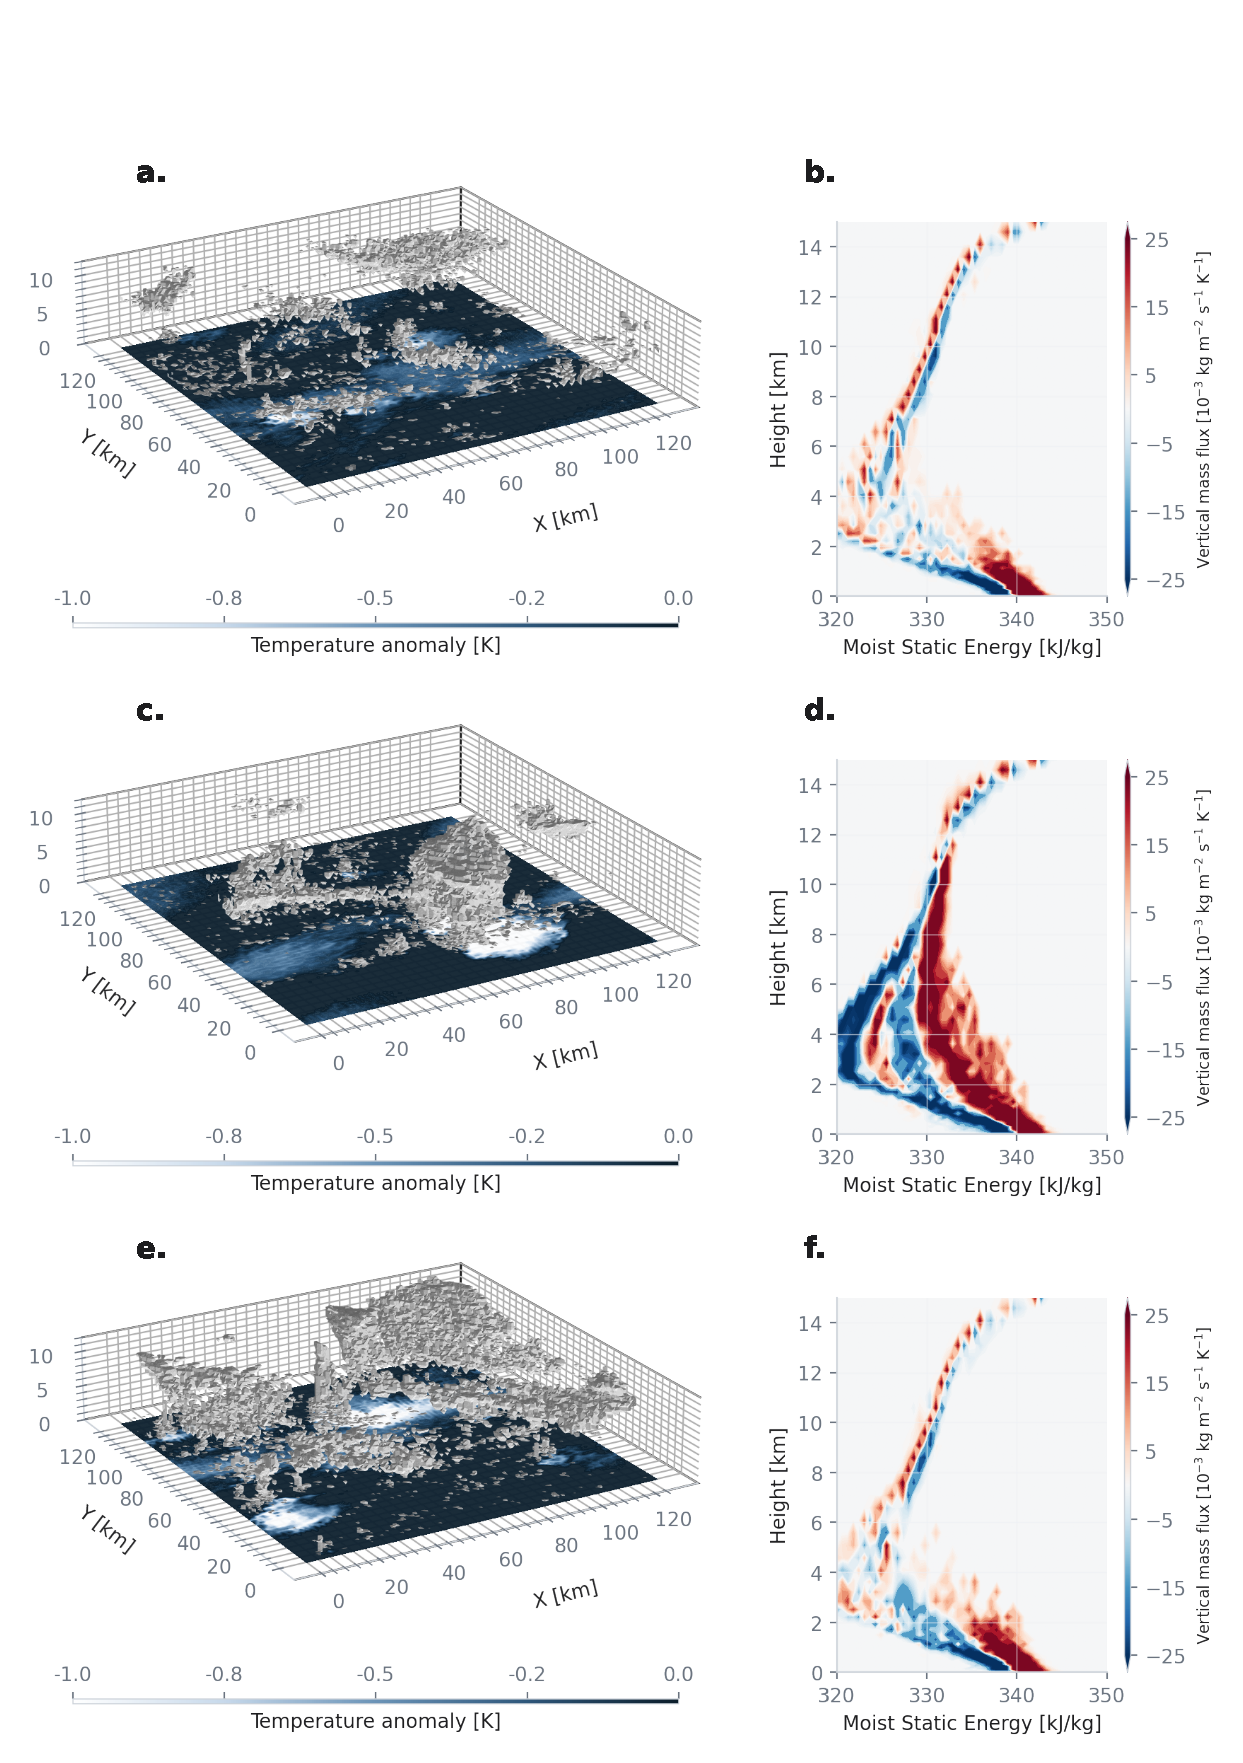
\includegraphics[width=0.8\linewidth]{fig1_snapshots.pdf}
    % \caption{A. Snapshot of the isovolume of non precipitating condensate (QN) at the levels 0f 0.02 kg/kg in volume and the surface temperature anomaly, the white zone corresponding to a cold pool. B. Time average over 27 days with 2min resolution of the isentropic mass flux.}
    \caption{\textbf{Three contrasting snapshots of the simulated convective field.} \textbf{Left (a, c, e):} isovolume of non-precipitating condensate $\mathrm{QN}=0.02$~kg\,kg$^{-1}$ over the surface temperature anomaly; white patches mark cold pools. \textbf{Right (b, d, f):} corresponding isentropic mass-flux diagram $M(h,z,t)$, with red (blue) indicating upward (downward) transport. \textbf{(a--b)} Suppressed: scattered shallow clouds, weak low-level transport. \textbf{(c--d)} Organized deep convection: a dominant tower with anvil and cold pool, sustained high-$h$ updrafts paired with low-$h$ downdrafts. \textbf{(e--f)} Unorganized active: many disconnected cells, diffuse mass-flux signatures.}
    \label{fig:simu_isentrop}
\end{figure}

The learning dataset is constructed from the time series of isentropic mass flux fields spanning 27 days with 2-minute temporal resolution. Moist static energy $h$ is discretized into 48 bins ranging from 320 to 350~kJ~kg$^{-1}$, and the vertical coordinate corresponds to the first 48 model levels, spanning altitudes from approximately 25~m to 16~km. The resulting raw dataset has dimensions $(n_t \approx 2\times10^{4},\, n_h=48,\, n_z=48)$. For each spatial pixel, the temporal mean is removed to suppress the stationary background signal and isolate transient variability. A spatial mask is then applied to retain only pixels that exhibit nonzero values at least once over the full time series, thereby discarding invariant regions of the domain; this is particularly important at higher altitudes, where the admissible range of $h$ progressively shrinks. The retained fields are subsequently reshaped into vectors. To enhance weak signals while preserving amplitude ordering, a signed logarithmic transform,
\[
\mathrm{sign}(x)\,\log(1+|x|),
\]
is applied to the masked values. The resulting mean-centered, masked, log-transformed vectors constitute the input representation used to train the model.

Given the time-ordered sequence of processed state vectors $\{X_t\}$, each training sample consists of a pair $(X_t, X_{t+\Delta t})$ separated by a fixed temporal offset $\Delta t = 5$. The full dataset is randomly permuted and split into a training set (90\%) and a validation set (9.9\%), with the remaining fraction excluded from optimization. During training, samples are drawn in mini-batches of size 256 and randomly shuffled at each epoch to decorrelate temporal ordering within batches, whereas the validation set is iterated deterministically.

\subsection{Reduced-order stochastic model}

The function of the designed model is not only to reduce the dimensionality of isentropic mass-flux diagrams, but to construct a dynamical, probabilistic representation of convective evolution. Specifically, we seek a reduced representation that (i) encodes the essential physical structure of convection, (ii) enables a meaningful partitioning of convective configurations into discrete states, and (iii) allows us to predict how convection is likely to evolve in time within this reduced space.

To this end, we introduce a reduced-order stochastic model that combines a variational autoencoder (VAE), a data-driven latent-state representation, and a discrete-time Markov transition model (Fig.~\ref{fig:model}). Rather than treating dimensionality reduction and temporal modeling as separate steps, the model is trained jointly so that the learned latent representation is both physically meaningful and dynamically predictive.

\begin{figure}
    \centering
    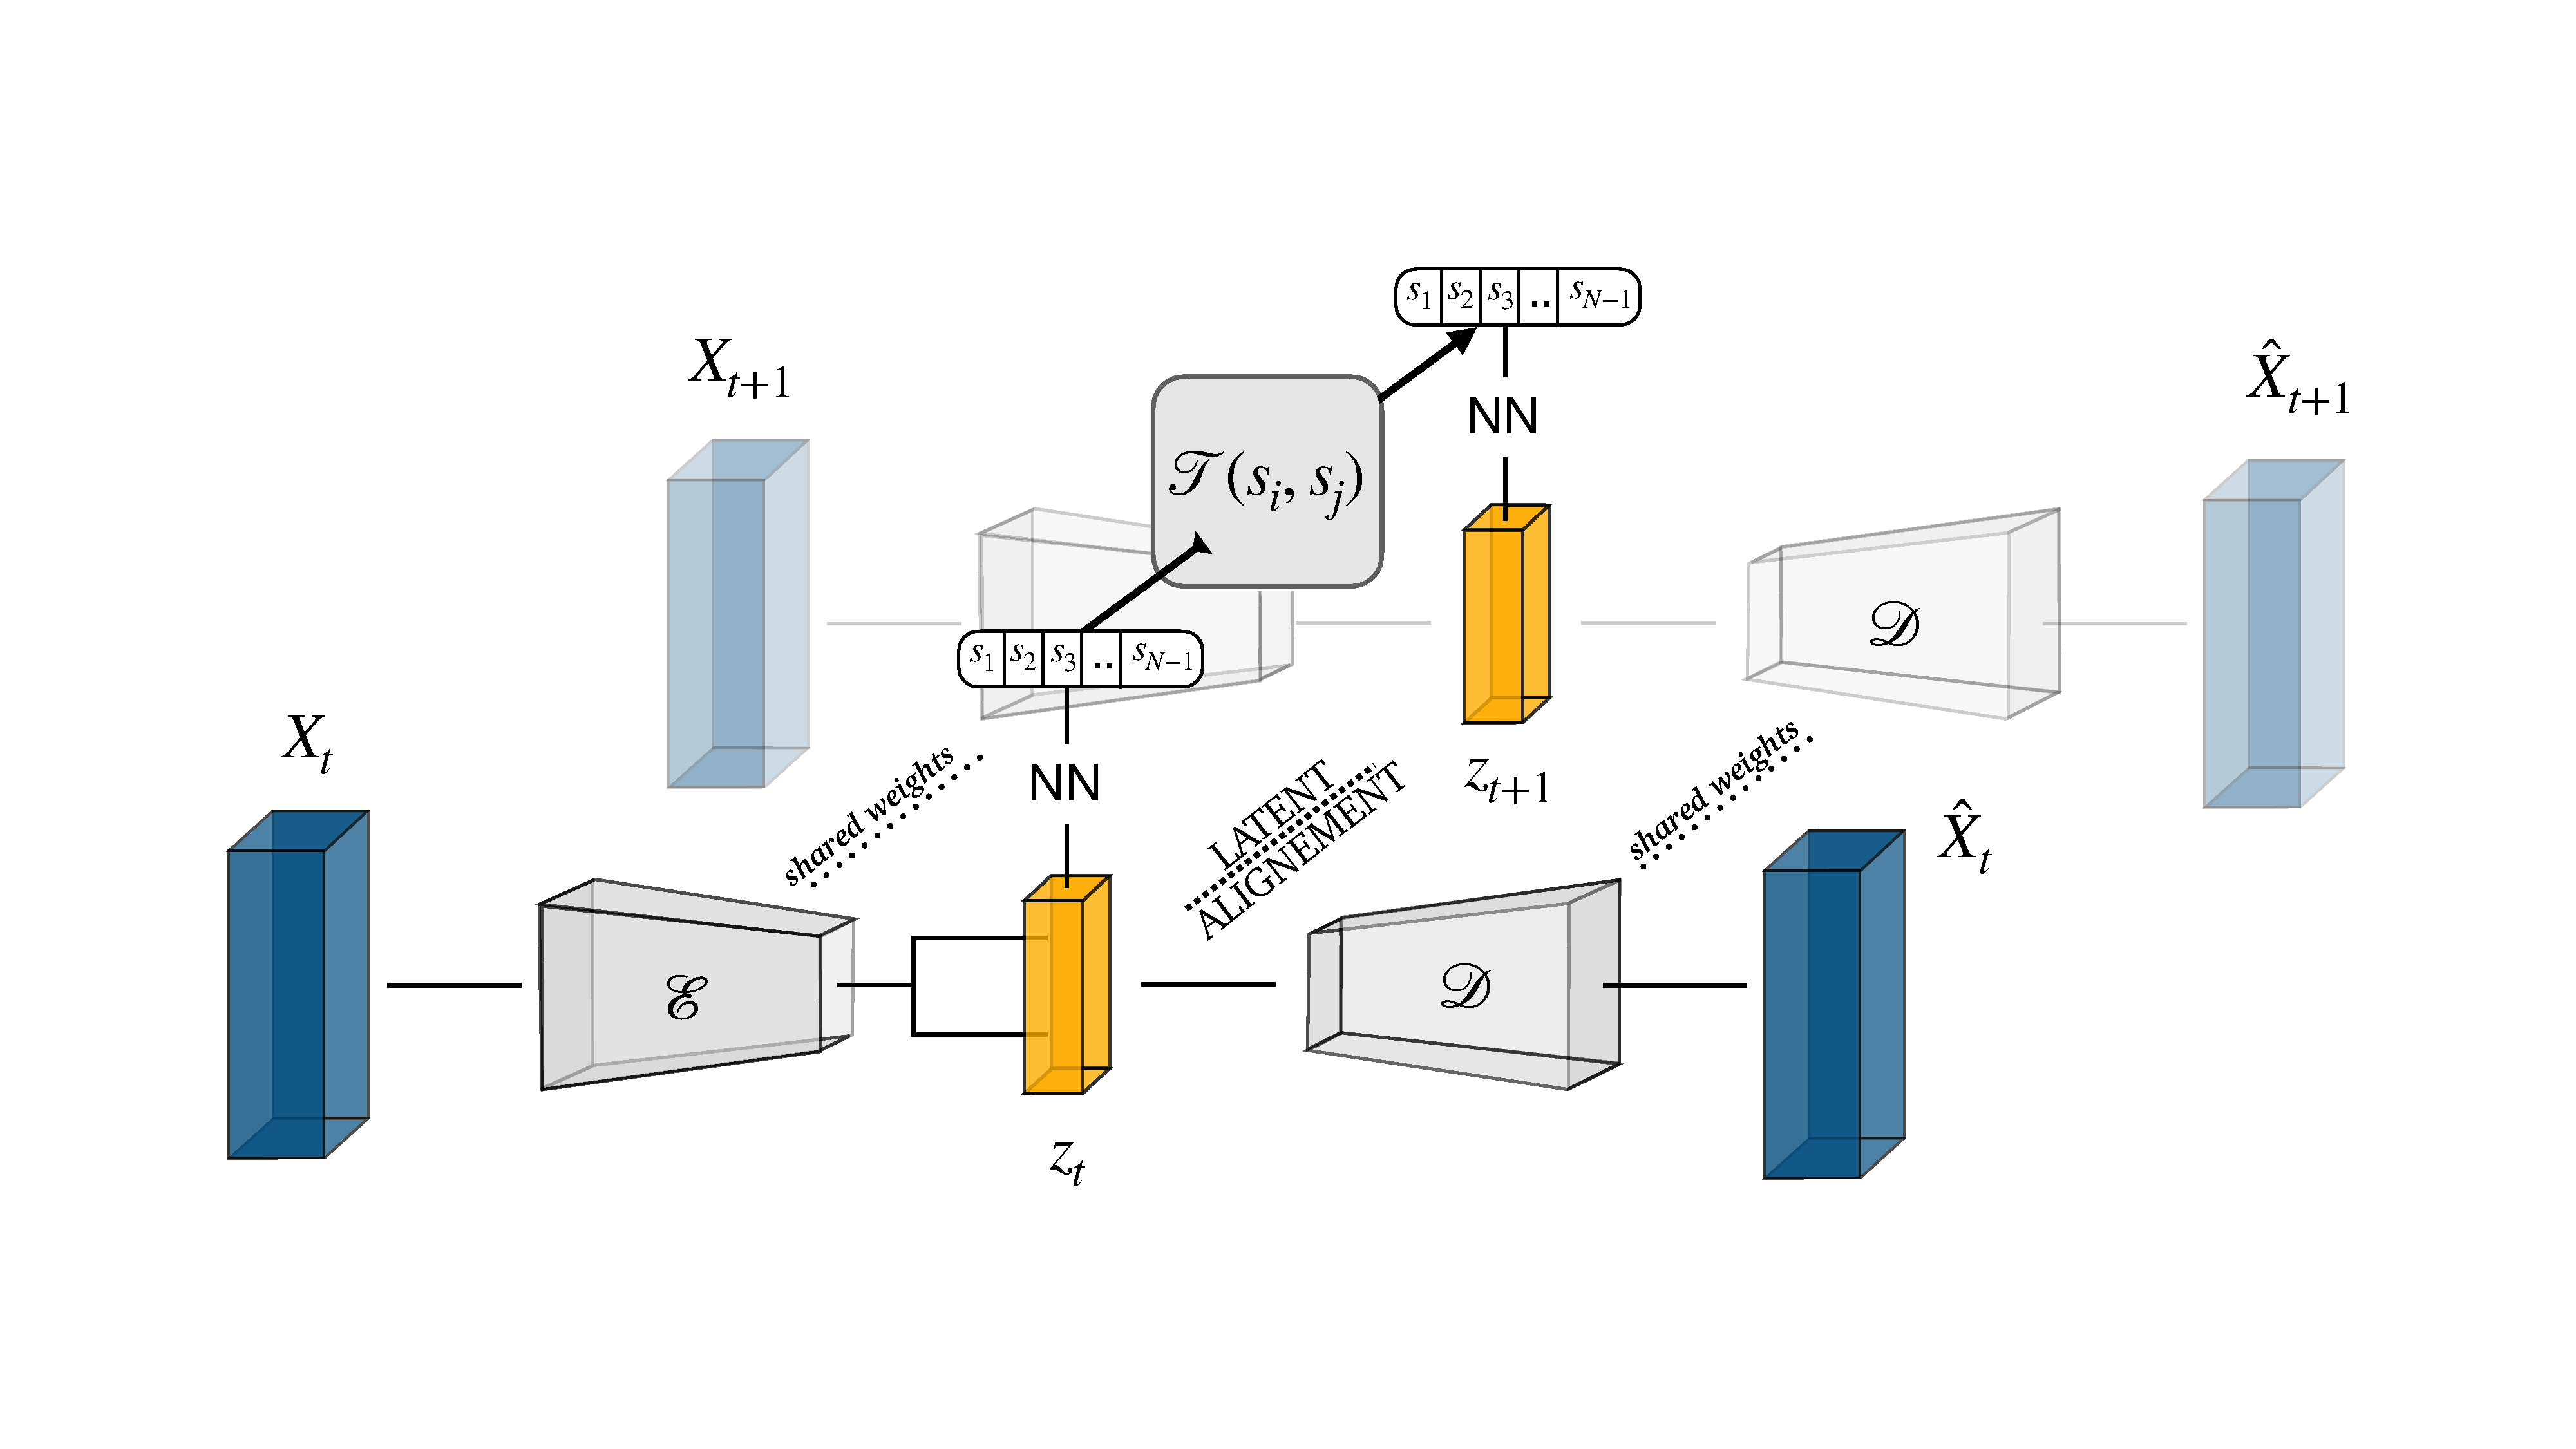
\includegraphics[width=0.9\linewidth]{model_vae_mc.pdf}
    \caption{\textbf{Model description.} The model combines a variational autoencoder (VAE) with a Markovian state assignment and transition framework. An encoder maps the input data to a latent representation $z_t$, which is reconstructed by a decoder. A neural network assigns to each latent vector $z_t$ a probability distribution over a finite set of discrete states. Temporal evolution in latent space is modeled by a linear transition operator $T$, which predicts the state distribution at time $t+1$ from the state distribution at time $t$. During training, consecutive latent vectors $(z_t, z_{t+1})$ are jointly considered: the VAE is trained using a reconstruction loss, while the transition operator is trained by comparing the predicted state distribution $T\,s(z_t)$ with the state distribution inferred from $z_{t+1}$.}
    \label{fig:model}
\end{figure}

\subsubsection{Variational autoencoder backbone}

Each isentropic mass-flux diagram at time $t$, denoted $X_t$, is encoded into a $d$-dimensional latent representation by a variational autoencoder. The encoder outputs a diagonal Gaussian posterior over the latent variable $z\in\mathbb{R}^d$,
\[
q(z \mid X_t) = \mathcal{N}\!\left(\mu(X_t),\,\mathrm{diag}(\sigma^2(X_t))\right),
\]
where $\mu(X_t)$ and $\sigma(X_t)$ are the mean and standard-deviation vectors produced by the encoder network. A latent sample $z\sim q(z|X_t)$ (drawn via the reparameterization trick) is decoded to produce a reconstruction $\hat{X}_t$, and reconstruction fidelity is enforced through the per-pixel summed squared error $\|X_t-\hat{X}_t\|^2$. The learned posterior is regularized toward an isotropic standard-Gaussian prior $p(z)=\mathcal{N}(0,I)$ through the closed-form Kullback--Leibler divergence $D_{\mathrm{KL}}(q\|p) = \tfrac{1}{2}\sum_{i=1}^d\!\left(\mu_i^2+\sigma_i^2-\log\sigma_i^2-1\right)$. This term enters the total objective with a small weight $\beta$ (Supplementary Information): it does not strongly compete with reconstruction fidelity, but it suffices to regularize the latent space so that the learned latent vectors are approximately Gaussian-distributed.

\subsubsection{Latent Space Partitioning}

The continuous latent representation is mapped onto a finite set of $K=5$ discrete convective states through a small neural network that takes $z_t$ as input and outputs a probability vector via a softmax head, $s_t = \mathrm{softmax}(g(z_t)) \in \Delta^{K-1}$, with $s_t(k)\ge 0$ and $\sum_k s_t(k)=1$. The number of clusters $K$ is set empirically (cluster-count sensitivity in Fig.~\ref{fig:cluster_sensitivity}). This mapping can be interpreted as a data-driven clustering mechanism, in which close latent representations are grouped into dynamically meaningful regimes. Importantly, because the clustering network is trained jointly with the encoder, it does not merely partition a fixed latent space but actively reshapes the latent geometry to favour cluster-consistent representations. The assignment is probabilistic rather than deterministic, allowing for uncertainty and overlap between states, which is essential in transitional or weakly organized configurations.

To prevent state collapse—whereby most samples are assigned to a small subset of states—we regularize the state assignment using a contrastive objective that encodes prior physical knowledge about the input. Specifically, we introduce a contrastive loss based on the structural similarity of isentropic mass-flux anomaly fields. Each sample is discretized into three regions using fixed thresholds $\{-1.5,\,1.5\}$, corresponding to negative anomalies, near-neutral values, and positive anomalies. From these regions, binary masks are constructed and compared using a macro-averaged Dice coefficient, which measures the spatial overlap of positive and negative anomaly structures while intentionally discarding information about anomaly amplitude or fine-scale intensity. For randomly sampled pairs $(i,j)$ within a batch, the Dice similarity $\mathrm{Dice}(i,j)$ defines a notion of physical proximity. Pairs with high structural similarity are encouraged to share the same latent state, while structurally dissimilar pairs are encouraged to occupy different states. This is implemented through a soft contrastive loss that penalizes disagreement for similar pairs (cohesion) and agreement for dissimilar pairs (separation), with a smooth transition between the two regimes. An additional mid-range penalty discourages uncertain assignments when the similarity is ambiguous. We denote this term as $\mathcal{L}_{\mathrm{Dice}}$ and adopt the convention that it is a \emph{similarity score} (larger when state assignments match the Dice-based structural similarity); accordingly, it enters the total loss with a negative sign so that maximizing similarity \emph{minimizes} the total objective. Full definition in Supplementary Information.

\subsubsection{Markov transition dynamics}

We assume that, at the temporal resolution of the simulations, the evolution of convection can be approximated as a first-order Markov process in state space. The transition probabilities are encoded in a transition matrix $T$, defined by
\[
T_{ij} = P(s_{t+\Delta t} = j \mid s_t = i),
\]
with rows that are non-negative and sum to unity (row-stochastic). The data are sampled every $\Delta t_\text{raw}=2\,\mathrm{min}$, but we evaluate transitions at $\Delta t = 5\,\Delta t_\text{raw} = 10\,\mathrm{min}$ (motivated in Section~\ref{sec:markov}). This matrix captures the persistence of convective regimes, preferred transitions, and rare events such as the onset or decay of organized convection. During training, the model receives frame pairs $(X_t, X_{t+\Delta t})$, encodes them into $(z_t, z_{t+\Delta t})$, and assigns states $(s_t, s_{t+\Delta t})$; $T$ is then fit so that $\hat{s}_{t+\Delta t} = T\, s_t$ matches $s_{t+\Delta t}$.

\subsubsection{Joint optimization}

The VAE, state-assignment network, and transition matrix are trained jointly by minimizing
\[
\mathcal{L} =
\underbrace{\|X - \hat{X}\|^2}_{\text{reconstruction}}
+
\underbrace{\tfrac{1}{2}\sum_{i=1}^d \left(\mu_i^2 + \sigma_i^2 - \log \sigma_i^2 - 1\right)}_{\text{KL to } \mathcal{N}(0,I)}
-
\underbrace{\mathcal{L}_{\mathrm{Dice}}}_{\text{contrastive}}
-
\underbrace{\sum_{i,j} s_t(i)\, s_{t+1}(j)\, \log T_{ij}}_{\text{transition log-likelihood}}.
\]
Each term is weighted by a non-negative coefficient ($\beta$, $\lambda_{\mathrm{Dice}}$, $\gamma_{\mathrm{MC}}$); values, together with encoder/decoder architectures, are reported in the Supplementary Information.

These four terms exert competing pressures on the latent geometry. The KL term pulls samples toward an isotropic Gaussian, while the Dice and transition terms favor a multi-modal structure in which samples cluster into $K$ regions separated by both structural similarity and temporal predictability. The resulting equilibrium is a latent space whose envelope remains approximately Gaussian but whose interior carries $K=5$ resolvable clusters (Fig.~\ref{fig:clusters}).

Optimization uses AdamW (learning rate $5\times10^{-5}$, batch size $256$) for $512$ epochs with gradient-norm clipping at $1.0$; the best model is selected by minimum validation loss. Loss decompositions (Fig.~\ref{fig:loss_curves}) and reconstruction diagnostics (Fig.~\ref{fig:reconstruction}) are provided in the Supplementary Information.



\section{Results}\label{sec:results}

\subsection{Physical interpretation of the latent space}

The model compresses time series of isentropic mass-flux fields---used here as a physically grounded representation of the convective state---into a time series of latent vectors $\mathbf{z}(t)\in\mathbb{R}^8$, with each time step assigned to one of five discrete convective states.

\paragraph{Latent-space structure revealed by PCA.}

A natural question is whether the latent space carries any physical meaning. There is no guarantee that it should: no physical constraint was imposed during training---the VAE is regularized only toward an isotropic Gaussian, and the five discrete states are assigned without reference to intensity, organization, or any other diagnostic. To probe the structure of the latent space, we apply PCA to the latent vectors $\mathbf{z}(t)$ and examine how the discrete clusters are arranged along its dominant modes of variability. The first two components explain $22\%$ and $17\%$ of the variance, respectively (Fig.~\ref{fig:clusters}); a three-dimensional projection (Supplementary Information, Fig.~\ref{fig:pca_3d}) confirms that clusters overlapping in 2D are separated along higher-order components.

\begin{figure}
    \centering
    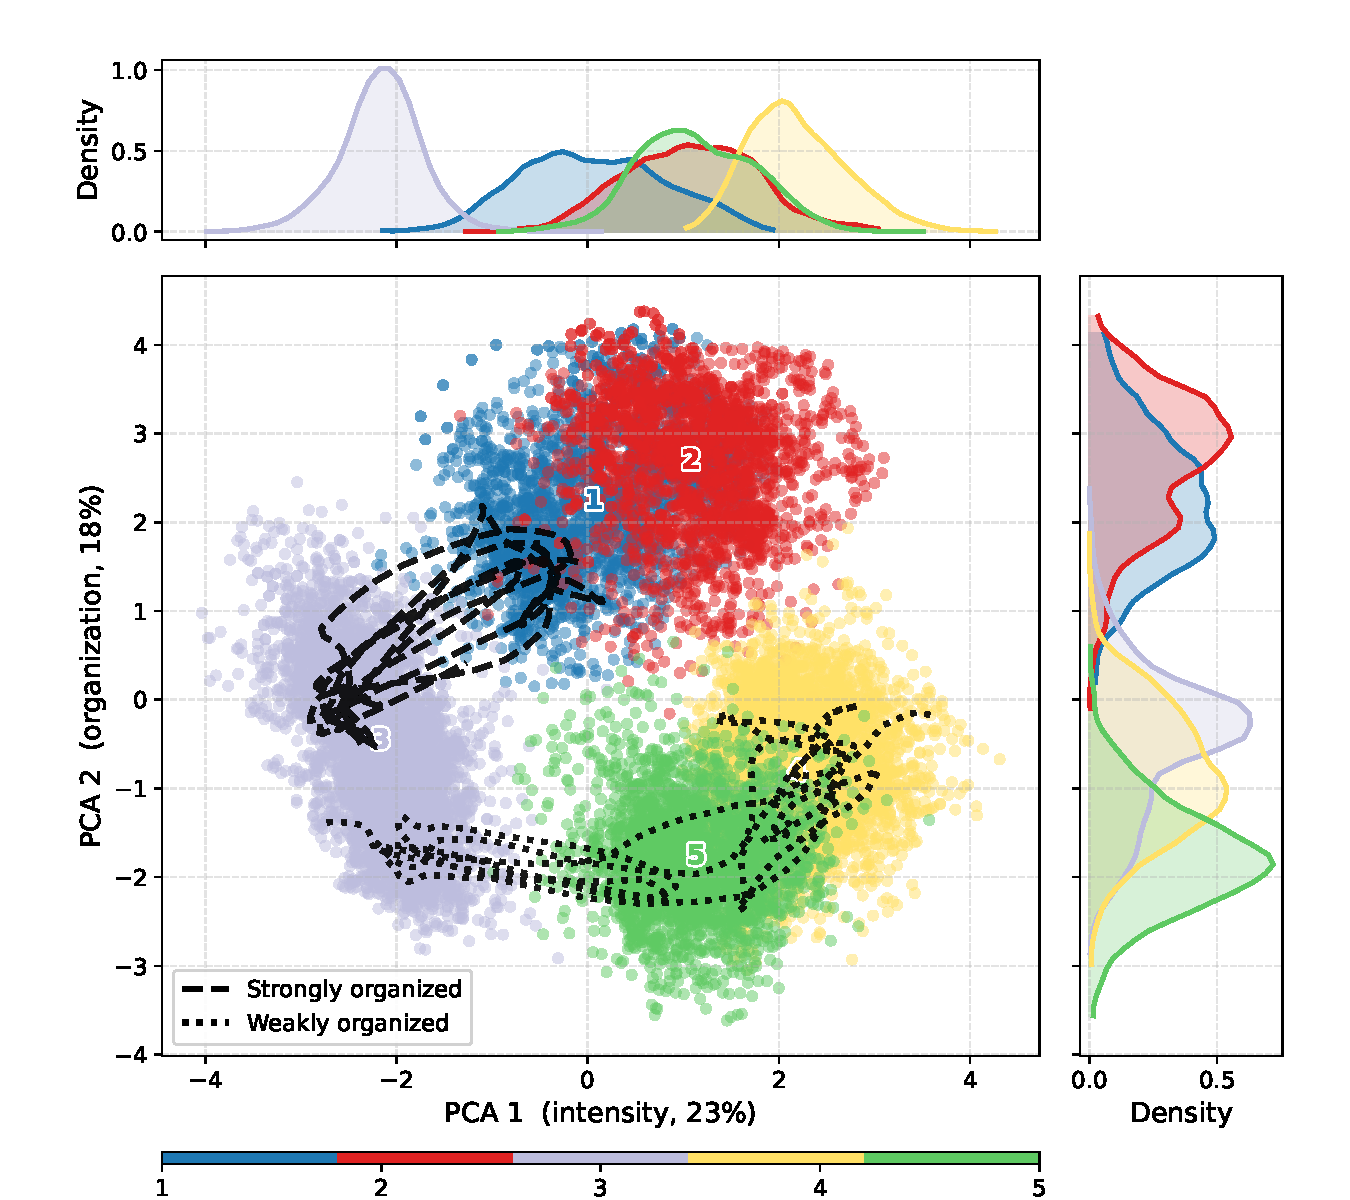
\includegraphics[width=0.75\textwidth]{fig3_clusters.pdf}
    \caption{\textbf{Latent-space organization.} PCA projection of the latent space colored by cluster assignment. Each point corresponds to one time step; trajectories illustrate the time evolution over 5~h.}
    \label{fig:clusters}
\end{figure}

\paragraph{Emergent axes: convective life cycle and organization.}

The physical interpretation of the dominant latent directions is obtained by relating the principal components to independent diagnostics of convection (Fig.~\ref{fig:axis_var}). The first principal component is strongly correlated with domain-mean precipitation, indicating that it primarily captures convective intensity and progression along the convective life cycle, from weak or suppressed states to vigorous, precipitating convection.

In contrast, the second principal component shows little correlation with precipitation but is strongly anticorrelated with a measure of cloud spatial organization derived from the variance of precipitable water. Variability along this axis therefore reflects differences in convective organization rather than intensity. The near-orthogonality of the two components indicates that convective intensity and spatial organization emerge as largely independent modes of variability in the learned representation.

\begin{figure}
    \centering
    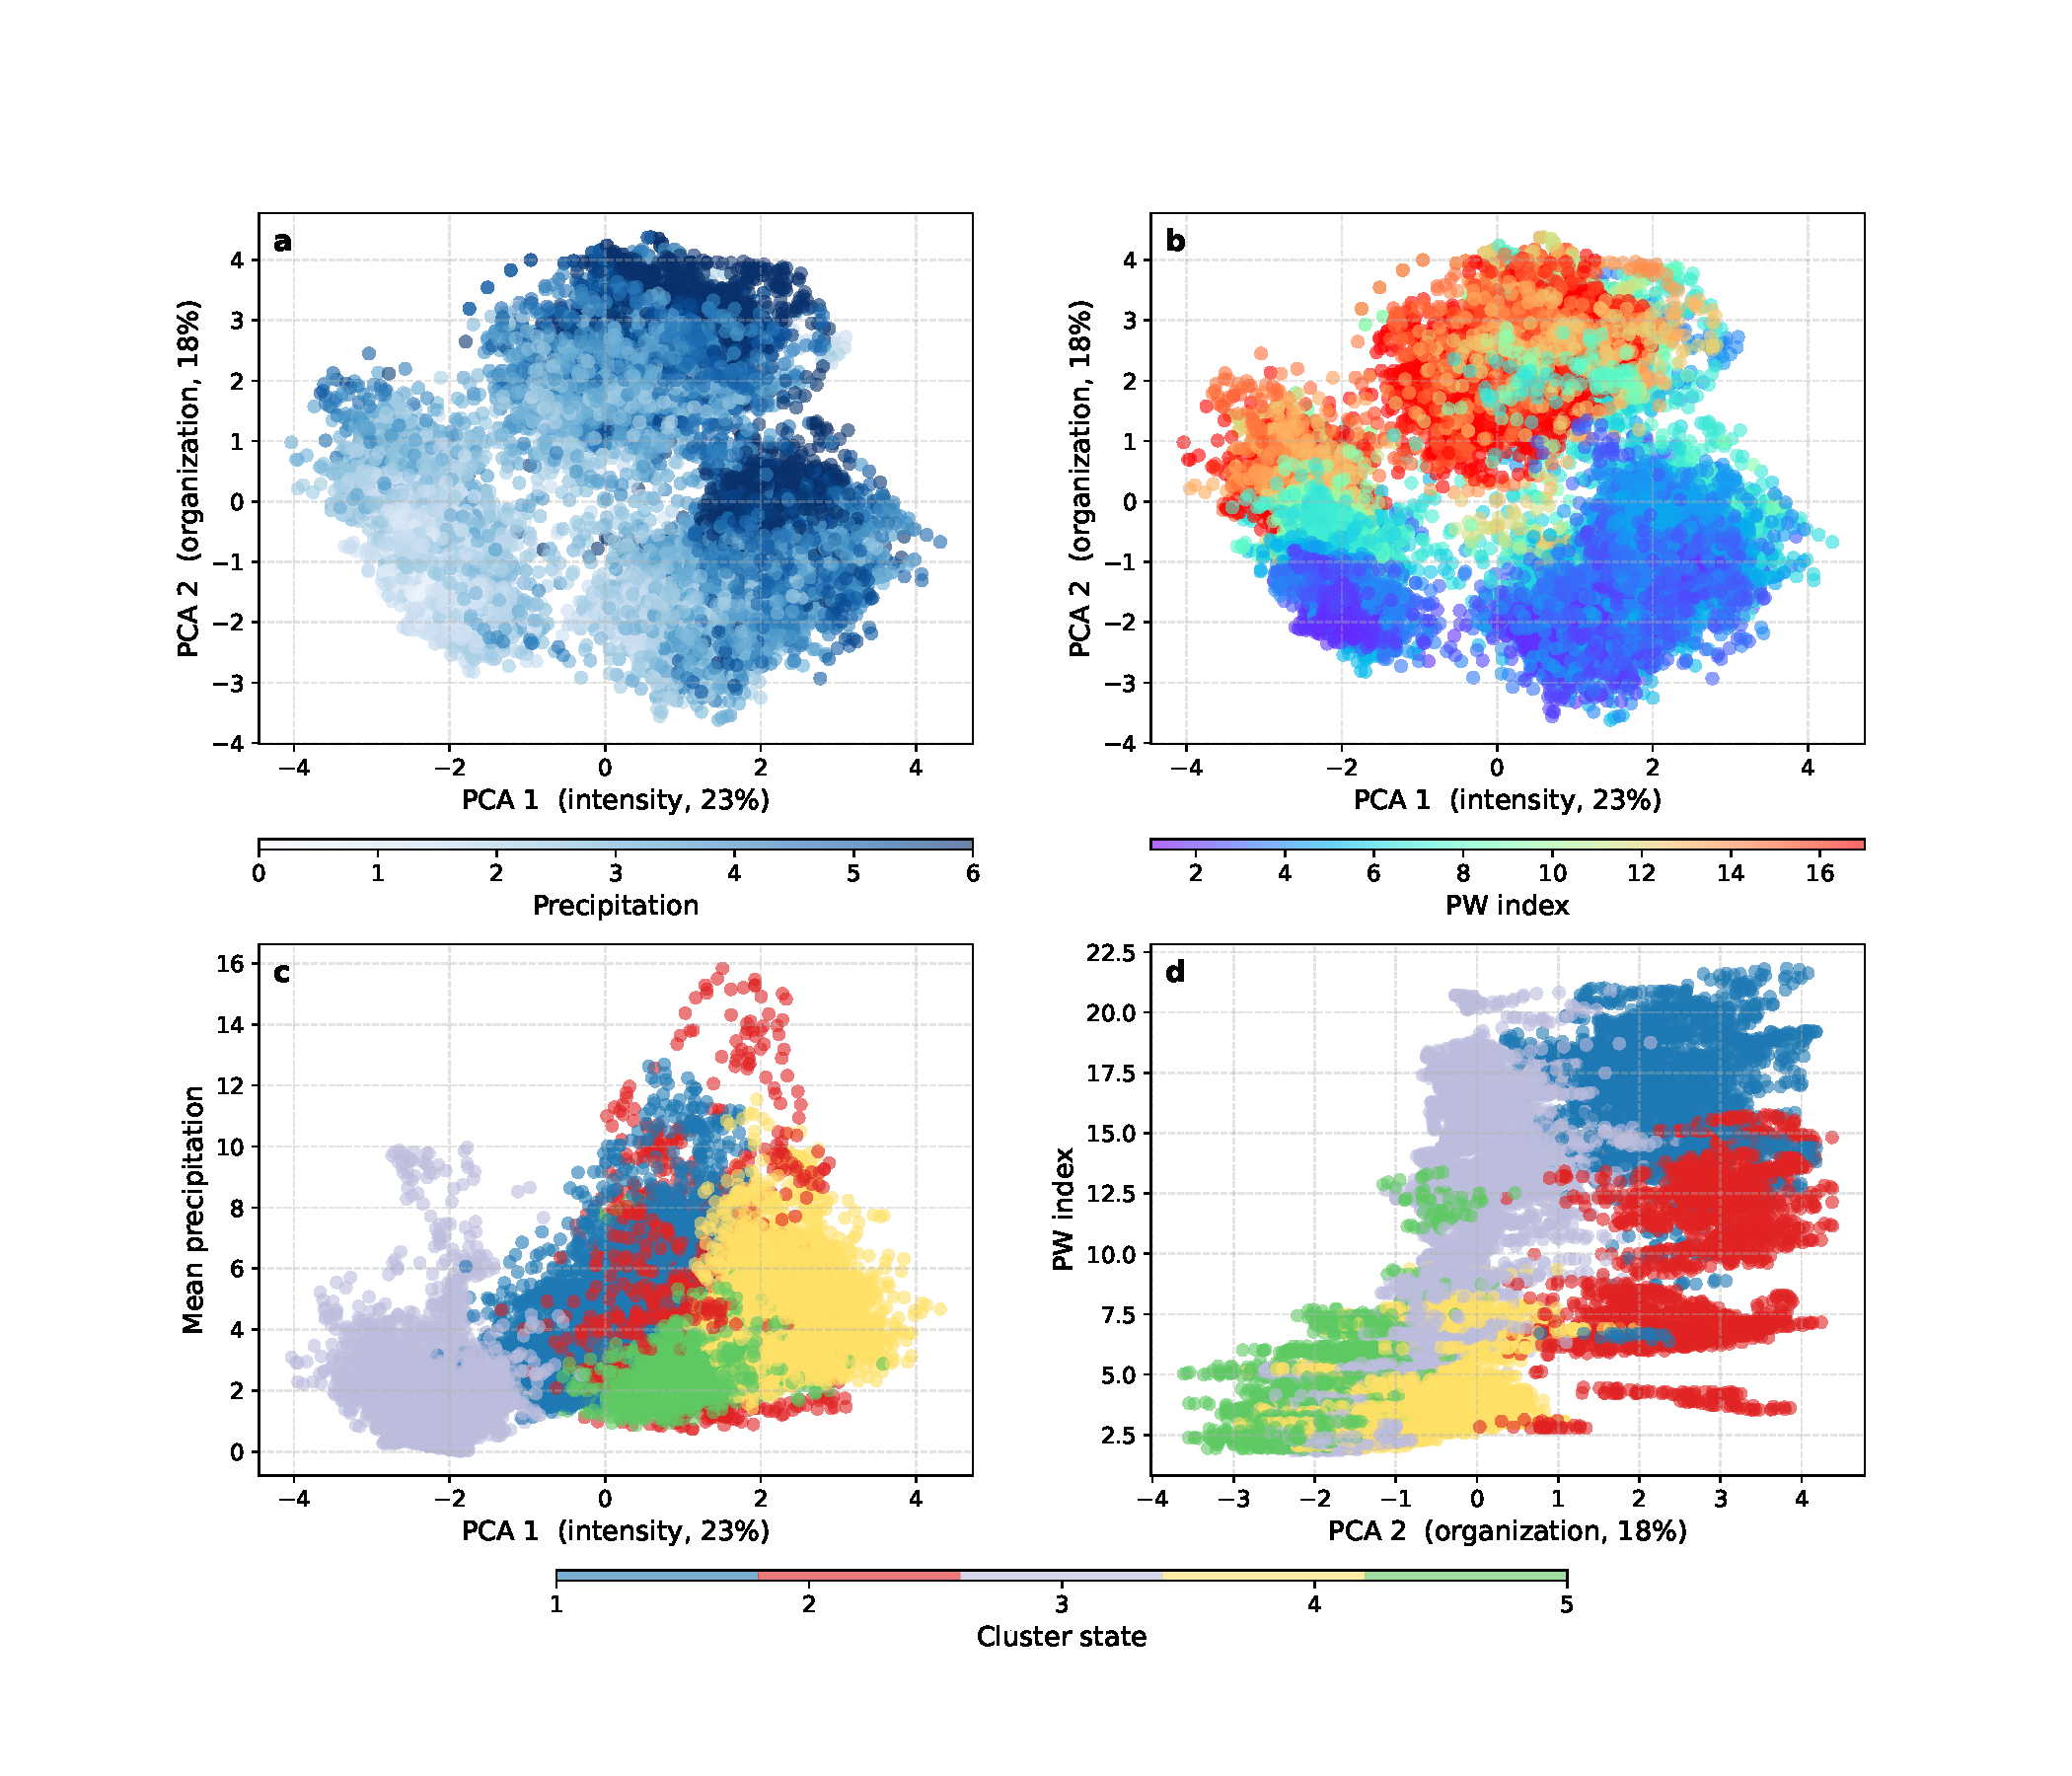
\includegraphics[width=0.95\linewidth]{fig4_latent_axis.pdf}
    \caption{\textbf{Physical interpretation of latent variability.} \textbf{(A)}~PCA projection coloured by the domain-mean precipitation, interpreted as a proxy for the intensity stage of the convective life cycle. \textbf{(B)}~PCA projection coloured by the variance of precipitable water (PW) over the domain, interpreted as a proxy for the spatial organization of the convective field: higher var(PW) corresponds to more clustered, organized convection. \textbf{(C--D)}~Joint distributions of the first two principal components against, respectively, the mean precipitation and the variance of PW.}
    \label{fig:axis_var}
\end{figure}

\paragraph{Dynamical and thermodynamic signatures of latent states.}

If the latent clusters correspond to physically meaningful convective regimes, they should be associated with systematic differences in vertical mass transport and thermodynamic structure. Representative isentropic mass-flux fields for each cluster are shown in Supplementary Information (Fig.~\ref{fig:state_means}).

Let $M(h,z,t)$ denote the isentropic mass flux at time $t$, height $z$, and moist static energy $h$. For each cluster $c$, we define the cluster-mean vertically integrated positive and negative mass fluxes,
\begin{equation}
M^{\pm}_c(z)
=
\left\langle
\int_h M(h,z,t)\,\mathbf{1}\{\pm M>0\}
\right\rangle_{t\in c},
\end{equation}
and the anomalies relative to the simulation-wide mean profiles $\overline{M}^{\pm}(z)$,
\begin{equation}
\Delta^{\pm}_c(z)
=
M^{\pm}_c(z)-\overline{M}^{\pm}(z).
\end{equation}

The resulting vertical profiles (Fig.~\ref{fig:vertical_profiles}) reveal sharp dynamical distinctions between clusters. Cluster~1 shows a positive (upward) anomaly extending through the deep troposphere with a comparatively weak negative (downward) anomaly at low levels, consistent with sustained deep ascent in a moist environment that suppresses lower-tropospheric detrainment. Cluster~2 shows an even stronger upper-tropospheric positive anomaly together with the deepest negative anomaly at mid-levels, the signature of a mature mesoscale-stratiform precipitation-driven system. Cluster~3 shows weak anomalies of either sign throughout the column. Cluster~4 shows strong positive and negative anomalies that peak at lower altitudes than Clusters~1--2, characteristic of active but weakly organized convection. Cluster~5 carries small positive anomalies confined to the lower troposphere over an otherwise weak deep-column signal, consistent with residual shallow convection in a suppressed environment.

\begin{figure}
    \centering
    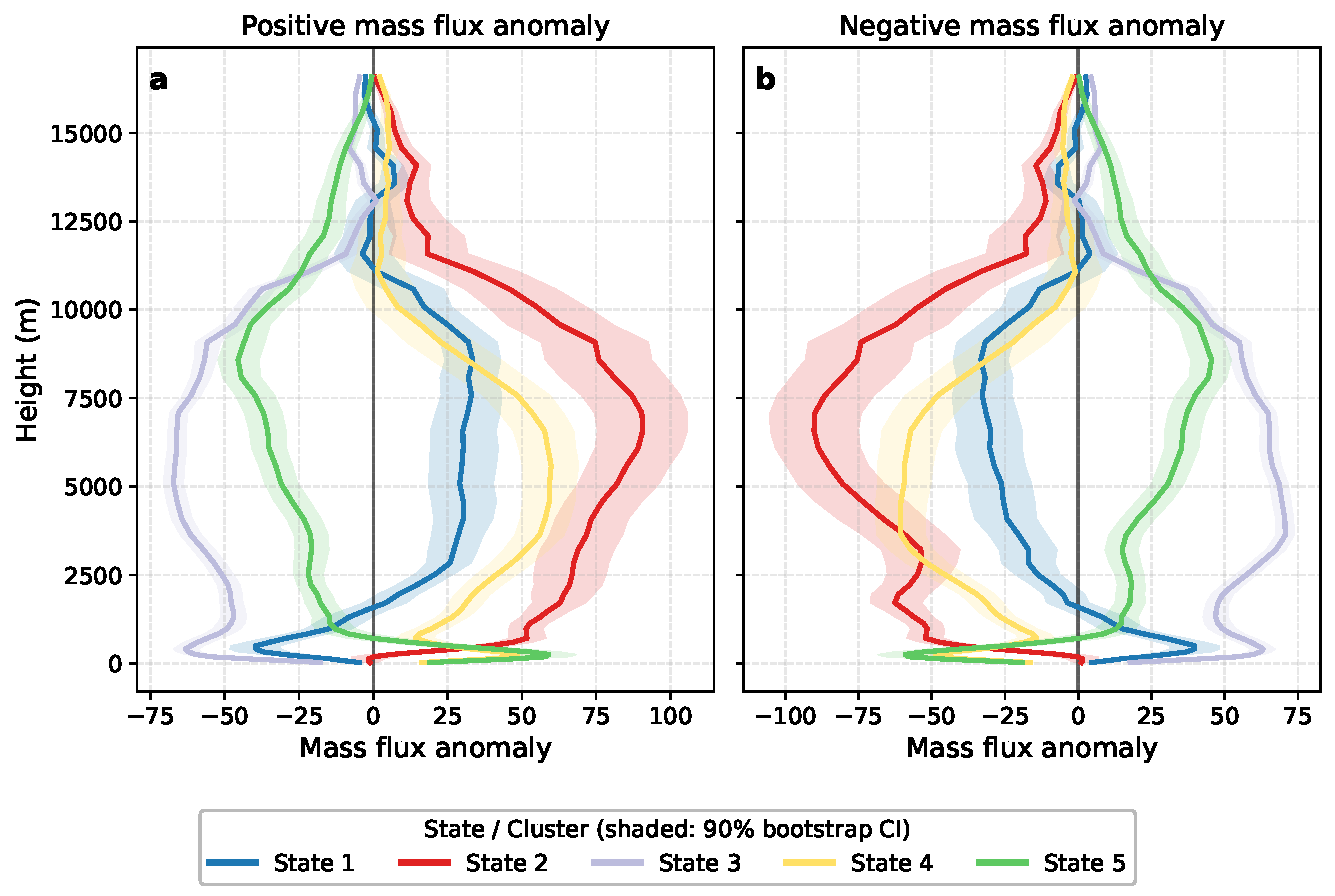
\includegraphics[width=0.8\textwidth]{fig5_vertical_profiles.pdf}
    \caption{\textbf{Cluster-averaged vertical mass-flux anomalies.} \textbf{(a)}~Positive (upward) and \textbf{(b)}~negative (downward) vertically resolved mass-flux anomalies relative to the simulation-wide mean profile $\overline{M}^{\pm}(z)$, computed from the samples closest to each cluster centroid in latent space. Each colour corresponds to one cluster (see legend); solid lines indicate the per-cluster mean, and shaded bands show the 90\% bootstrap confidence interval. A positive value at altitude $z$ means the cluster's upward (or downward) mass flux at that height exceeds the simulation-wide mean; a negative value means it lies below.}
    \label{fig:vertical_profiles}
\end{figure}

The distribution of mass-flux anomalies across moist static energy (Fig.~\ref{fig:mse_profiles}) reveals corresponding thermodynamic distinctions. Cluster~1 carries its strongest positive (upward) anomaly at high moist static energy ($\theta \approx 343$~K), consistent with the lifting of warm, moist air in a deep convective column with reduced entrainment. Cluster~2 carries strong positive and negative anomalies distributed broadly across the mid to high moist-static-energy range ($\theta \approx 330$--$345$~K), with the positive peak located at intermediate $\theta$ rather than at the highest values, the signature of detrainment into a mesoscale stratiform region. Cluster~3 lies below the simulation-wide mean across the entire moist-static-energy range, indicating an overall suppression of both upward and downward mass flux. Cluster~4 carries strong positive and negative anomalies concentrated at lower moist static energy ($\theta \approx 329$~K), consistent with the lifting of less buoyant air, stronger entrainment, and more transient convection. Cluster~5 carries weak anomalies localized to low--intermediate moist static energy with little upper-tropospheric signal, consistent with residual shallow activity in a drier column.

\begin{figure}
    \centering
    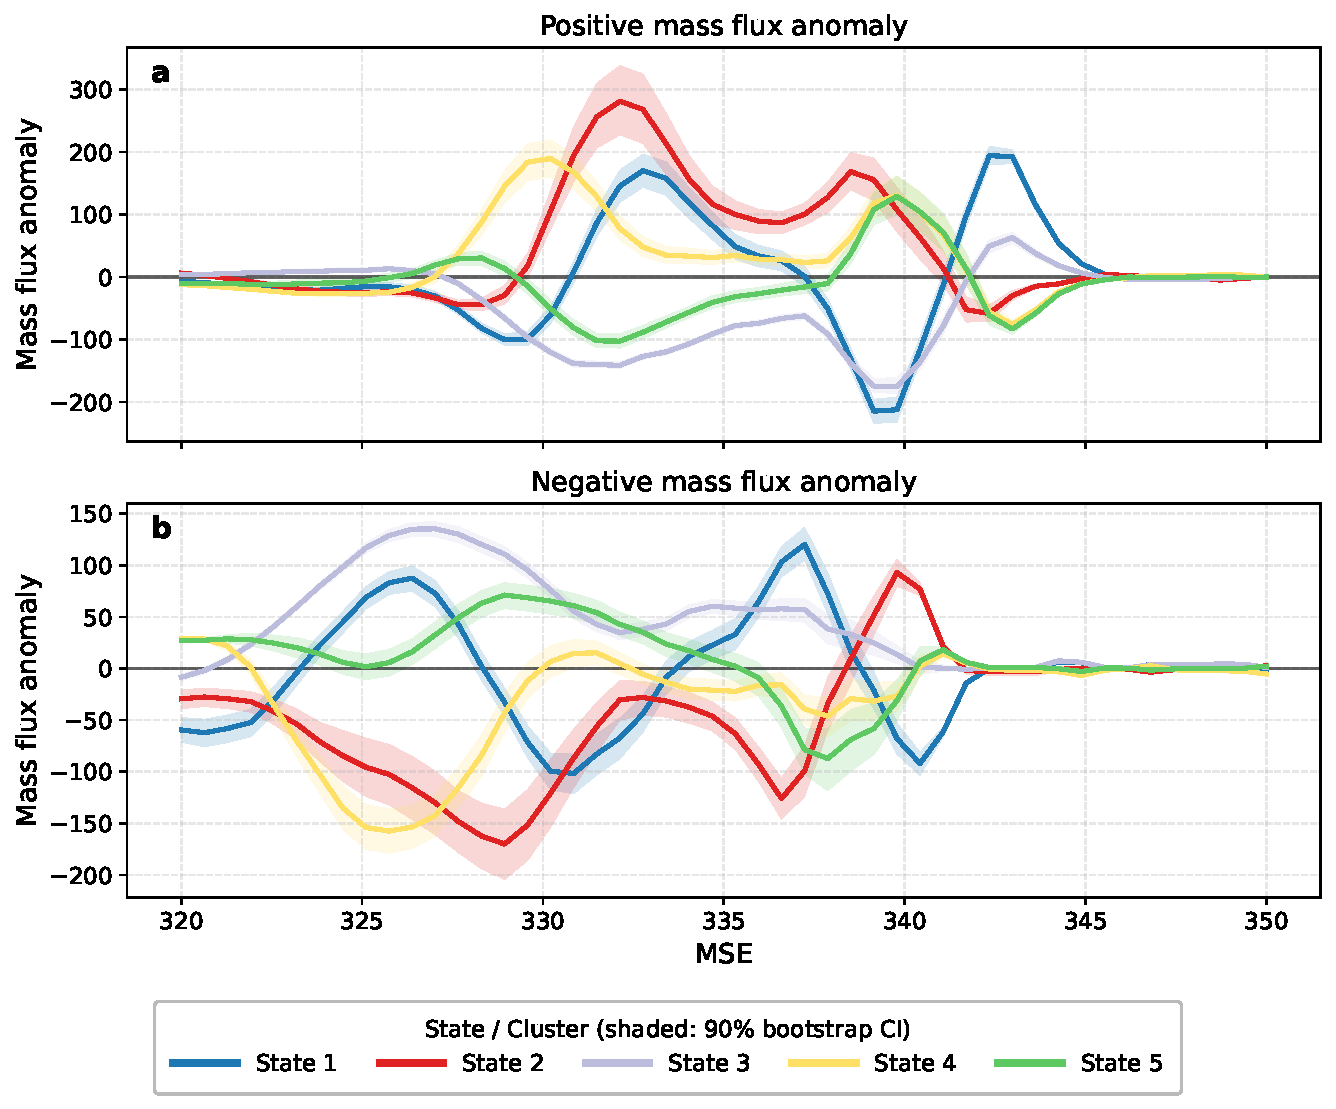
\includegraphics[width=0.8\textwidth]{fig6_mse_profiles.pdf}
    \caption{\textbf{Cluster-averaged mass-flux anomalies resolved along moist static energy.} \textbf{(a)}~Positive (upward) and \textbf{(b)}~negative (downward) mass-flux anomalies relative to the simulation-wide mean, computed from the samples closest to each cluster centroid in latent space and binned by moist static energy $\theta$. Each colour corresponds to one cluster (see legend); solid lines indicate the per-cluster mean, and shaded bands show the 90\% bootstrap confidence interval. A peak at a given $\theta$ identifies the moist-static-energy range across which the cluster's mass-flux activity is concentrated.}
    \label{fig:mse_profiles}
\end{figure}

Together, these results show that the VAE latent space organizes convective variability along two emergent and physically interpretable axes—intensity and organization—and that the resulting discrete latent states correspond to dynamically and thermodynamically distinct convective regimes. Table~\ref{tab:state_summary} consolidates the per-cluster numerical and physical characterization.

\begin{table}[t]
\centering
\small
\begin{tabular}{@{}c l c p{0.58\textwidth}@{}}
\hline
State & Name & $\pi$ (\%) & Physical signature \\
\hline
1 & \emph{Organized deep}     & 12.9 & sustained deep ascent in a moist environment; reduced low-level detrainment; highest precipitable water \\
2 & \emph{Stratiform-like}    & 12.2 & strongly active convection with large upper-tropospheric mass flux, consistent with a mesoscale stratiform region; highest precipitation \\
3 & \emph{Suppressed convection} & 37.0 & weak up- and down-drafts; dry background atmosphere; dominant state \\
4 & \emph{Active unorganized}     & 22.7 & active convection with mass flux peaking at lower altitudes than in the organized regime; drier environment \\
5 & \emph{Shallow congestus}      & 15.2 & suppressed deep convection with residual shallow convective activity; dry environment \\
\hline
\end{tabular}
\caption{\textbf{Summary of the five latent convective states.} Cluster identities are inferred from the interpretation of the latent-space axes of variability (Fig.~\ref{fig:axis_var}) and confirmed by the per-cluster vertical (Fig.~\ref{fig:vertical_profiles}) and moist-static-energy (Fig.~\ref{fig:mse_profiles}) mass-flux profiles. $\pi_i$ is the stationary probability of cluster~$i$ (Eq.~\ref{eq:canon}).}
\label{tab:state_summary}
\end{table}


\subsection{Markov transition matrix, eigenmodes, and regimes}

The second output of the model is a Markov transition matrix $\mathbf{T}$, whose elements
\begin{equation}
T_{ij} = \mathbb{P}\left( X_{t+\Delta t} = j \mid X_t = i \right)
\end{equation}
denote the probability of transitioning from state $i$ to state $j$. The resulting transition matrix is shown in Fig.~\ref{fig:markov_matrix}.

\begin{figure}
    \centering
    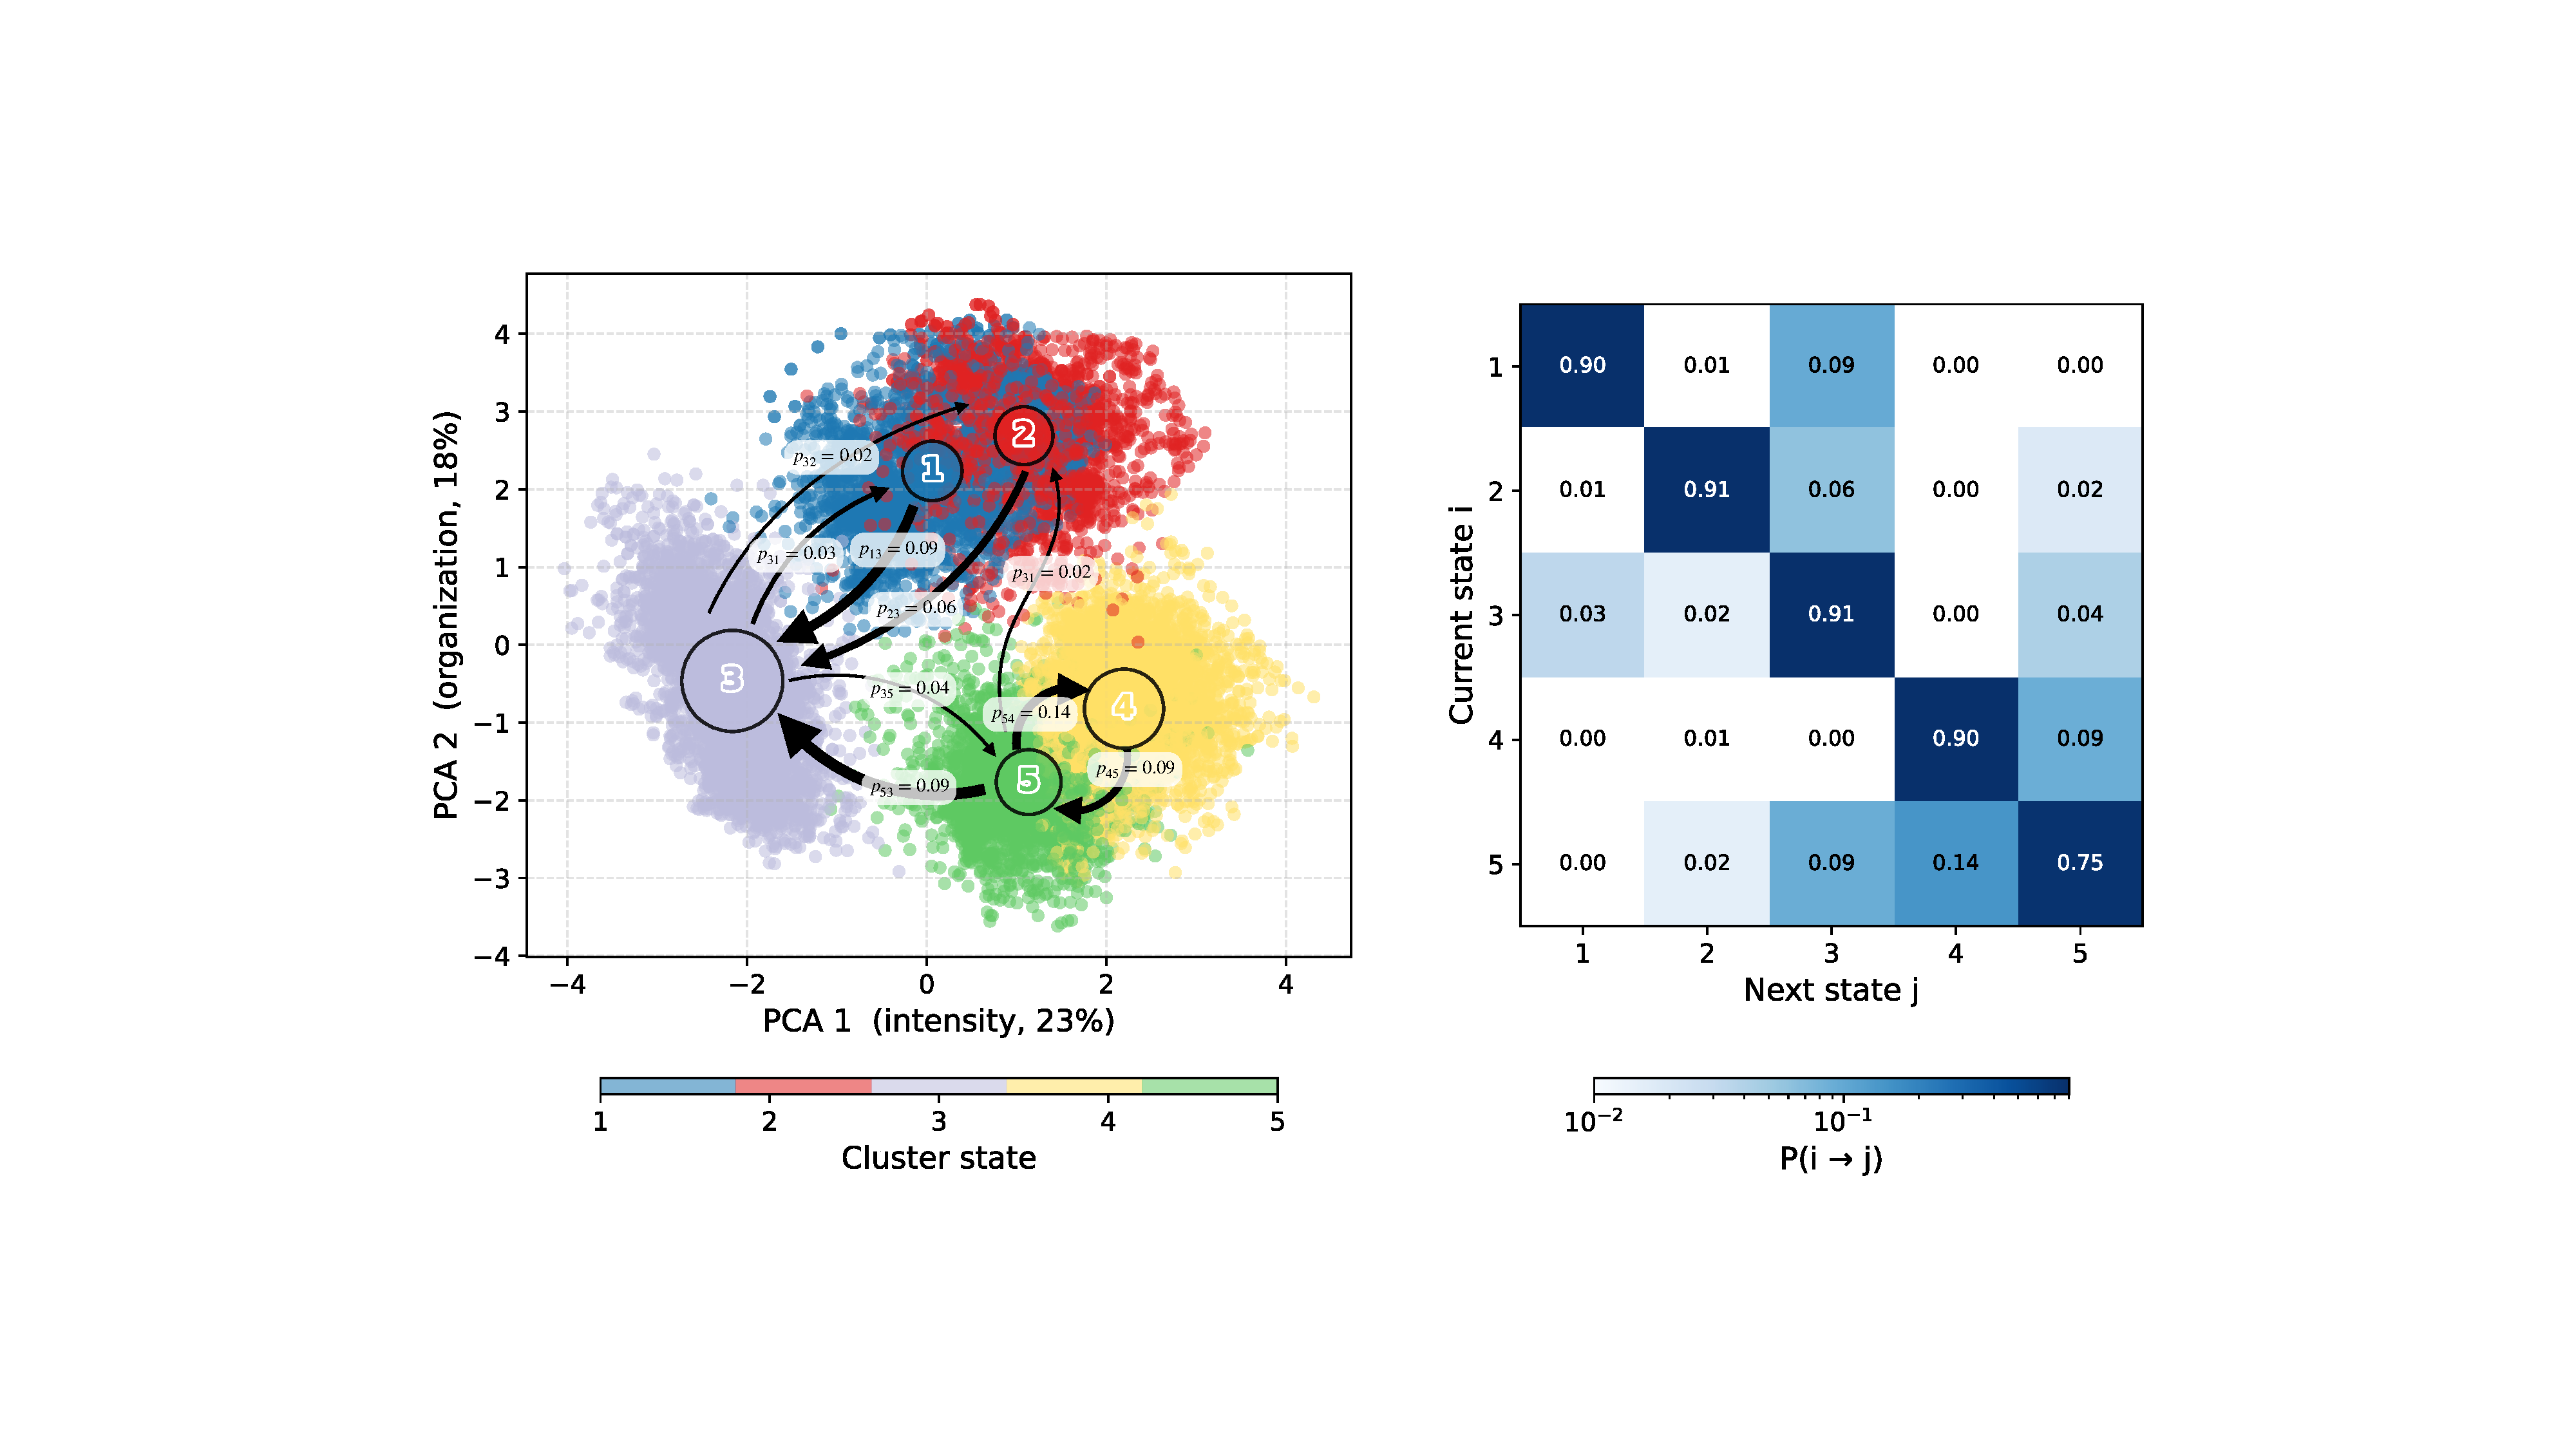
\includegraphics[width=\textwidth]{fig7_markov_matrix.pdf}
    \caption{\textbf{Markov state dynamics in latent space.} \textbf{(A)} Latent space visualization with the inferred Markov chain overlaid; example trajectories along the two dominant pathways are drawn on top (the corresponding time series are shown in Supplementary Information, Fig.~\ref{fig:trajectories}). The size of each state node is proportional to its asymptotic (stationary) probability, and arrows indicate transition probabilities between states. \textbf{(B)} Transition matrix describing the dynamics of convection under a given shear. The dominance of the diagonal indicates strong state persistence, with the system remaining in a given state for extended periods. Analysis of the transition structure reveals two coupled blocks separated by Cluster~3 (suppressed convection): Clusters~1--2 (the organized regime) and Clusters~4--5 (the unorganized regime).}
    \label{fig:markov_matrix}
\end{figure}

The matrix $\mathbf{T}$ is strongly diagonally dominated, indicating that the
system tends to persist within a given state over several time steps.
Moreover, the matrix is sparse, with only a limited number of preferred transitions
between states, suggesting constrained pathways in state space.

To further characterize the dynamics, we perform a spectral decomposition of
$\mathbf{T}$.
Because $\mathbf{T}$ is stochastic, it admits a unit eigenvalue $\lambda_1=1$. The corresponding right eigenvector $\boldsymbol{\pi}$ satisfies $\mathbf{T}\boldsymbol{\pi}=\boldsymbol{\pi}$ and defines the stationary distribution of the Markov chain. We obtain
\begin{equation}
\boldsymbol{\pi} =
\begin{bmatrix}
12.9\% & 12.2\% & 37.0\% & 22.7\% & 15.2\%
\end{bmatrix}.
\label{eq:canon}
\end{equation}

The stationary distribution is dominated by Cluster~3 ($37.0\%$, suppressed convection), with the remaining weight distributed across four substantially occupied states: Cluster~4 ($22.7\%$, active unorganized convection), Cluster~5 ($15.2\%$, shallow congestus), Cluster~1 ($12.9\%$, organized deep ascent), and Cluster~2 ($12.2\%$, stratiform-like deep convection). The five-state partition therefore concentrates the variability into a dominant suppressed background and four dynamically distinct active regimes, all sufficiently populated to constrain the inferred transition statistics.

We next examine the subdominant eigenvalues and eigenvectors of
$\mathbf{T}$.
All non-stationary eigenvalues have imaginary parts at the level of numerical noise ($|\mathrm{Im}(\lambda_k)|<10^{-3}$); the spectrum is effectively real. This indicates that the dominant dynamics cannot be described as simple linear oscillations in state space.

The leading nontrivial eigenvalue of the transition matrix is
\begin{equation}
\lambda_2 \approx 0.94,
\end{equation}
indicating a highly persistent dynamical mode. The corresponding eigenvector
\begin{equation}
\mathbf{v}_2 =
\begin{bmatrix}
-0.56 & -0.30 & -0.25 & +0.65 & +0.34
\end{bmatrix}
\end{equation}
(unit-norm; the overall sign is arbitrary). A positive $(\mathbf{v}_2)_i$ means cluster~$i$ is enhanced relative to $\pi_i$ in one phase of this mode and suppressed in the other; $|(\mathbf{v}_2)_i|$ sets the relative size of that deviation across clusters. Components of opposite sign therefore vary in anti-phase.

The components of $\mathbf{v}_2$ split the chain into two opposite-sign groups, $\{1,2\}$ ($-0.56,\,-0.30$) and $\{4,5\}$ ($+0.65,\,+0.34$); Cluster~3 has the smallest amplitude in this mode ($-0.25$). We interpret these two groups as two convective regimes---\emph{organized} ($\{1,2\}$) and \emph{unorganized} ($\{4,5\}$)---that the chain alternates between on the eigenmode decay time $\tau_2 = -\Delta t / \log|\lambda_2| \approx 172\,\mathrm{min}$. Cluster~3, despite its small amplitude in $\mathbf{v}_2$, carries the dominant stationary occupancy ($\pi_3=37\%$), and nearly every transition between the other four clusters passes through it (Fig.~\ref{fig:markov_matrix}b); it therefore functions as the chain's intermediate state, visited routinely between successive episodes in the other clusters.

The internal dynamics of the two regimes differ. The unorganized regime is a closed oscillation: Clusters~4 and~5 exchange directly and frequently ($T_{4\to 5}=0.09$, $T_{5\to 4}=0.14$). The organized regime is not. Clusters~1 and~2 do not exchange directly ($T_{1\to 2}=T_{2\to 1}=0.01$), and they are also separated in time: $200$~min after a Cluster-1 timestep, the conditional probability of being in Cluster~2 is $0.04$, well below the stationary value $\pi_2=0.12$. Cluster~1 (deep moist ascent, reduced low-level detrainment) and Cluster~2 (mesoscale stratiform-like deep convection) therefore appear as independent organized episodes, each returning to Cluster~3 before the next can begin. Time series of individual realizations (Supplementary Information, Fig.~\ref{fig:trajectories}) reflect this: organized intervals are dominated by a $3\!\leftrightarrow\!1$ oscillation with occasional Cluster-2 excursions, while unorganized intervals follow the $3\!\leftrightarrow\!5\!\leftrightarrow\!4$ cycle.

The eigenvalue spectrum just identified makes a quantitative prediction: for a true Markov chain, the autocorrelation of every state's occupancy must be a sum of exponentials with the decay times $\tau_k = -\Delta t / \log|\lambda_k|$. In the next subsection we test this prediction directly against the empirical autocorrelations, identifying which states deviate from Markovian behavior and how those deviations reveal internal feedbacks such as cold-pool memory.


\subsection{Markovianity assessment and internal feedbacks}\label{sec:markov}

We now ask whether the five-state chain is self-contained --- whether the state at time $t$ alone determines the distribution at $t+\tau$. Departures from this Markov property identify slow internal processes (moisture memory, cold pools, mesoscale organization) that the partition does not resolve. The question is long-standing: classical convective parameterizations assume instantaneous quasi-equilibrium adjustment \citep{zhang2003convective, bechtold2014representing}, while more recent schemes introduce explicit memory variables to capture lagged responses \citep{piriou2007approach, gerard2009cloud, mapes2011parameterizing, hwong2023assessing}.

\paragraph{Indicator autocorrelation.}
Defining the occupancy indicator $I_i(t) = \mathbf{1}[X_t = i]$ and its normalized autocorrelation
\begin{equation}
C_i(\tau) =
\frac{\mathbb{E}\!\left[(I_i(t)-\pi_i)(I_i(t+\tau)-\pi_i)\right]}
     {\mathbb{E}\!\left[(I_i(t)-\pi_i)^2\right]},
\end{equation}
a discrete-time Markov chain with transition matrix $\mathbf{T}$ and stationary distribution $\boldsymbol{\pi}$ admits the closed form \citep{souza2024representing}
\begin{equation}
C_i(\tau) \;=\; \frac{T^\tau_{ii} - \pi_i}{1-\pi_i}
\;=\; \sum_{\alpha=2}^K A_\alpha^{(i)}\, \lambda_\alpha^\tau,
\label{eq:autocor}
\end{equation}
a superposition of exponentially decaying modes set by the eigenvalues $\lambda_\alpha$ of $\mathbf{T}$, with state-dependent amplitudes $A_\alpha^{(i)} = (\mathbf{v}_\alpha)_i (\mathbf{w}_\alpha)_i / (1-\pi_i)$, where $\mathbf{v}_\alpha$ and $\mathbf{w}_\alpha$ are the right and left eigenvectors of $\mathbf{T}$ (derivation in SI). Departures from this prediction quantify residual memory not encoded by the partition.

\paragraph{Memory beyond Markov in the convection-active states.}
Most clusters' empirical autocorrelations track the Markov prediction of Eq.~\ref{eq:autocor}: in Fig.~\ref{fig:autocorrelation}a, the solid (empirical) and same-colour dashed (Markov) curves overlap to within noise. Two clusters deviate visibly. The organized Cluster~1 (blue) sits noticeably above its Markov prediction throughout the lag window, followed by the active-unorganized Cluster~4 (yellow); Cluster~3 (suppressed convection) tracks its prediction most closely. This distinction matters: a state can be \emph{sustained} (long dwell times) and still \emph{Markovian} if its diagonal $T_{ii}$ alone explains the persistence; Clusters~1 and~4 are sustained \emph{beyond} what $T_{ii}$ predicts, indicating that an internal degree of freedom not represented in the partition is keeping them alive.

\paragraph{Cold pools partly close the gap.}
Cold pools are a natural candidate carrier of this missing memory \citep{tompkins2001coldpools, houze1977structure, rotunno1988theory}. The hypothesis is testable: if cold pools carry the memory, then knowing the cold-pool field at the starting time should make the subsequent Cluster~1 dynamics more Markovian---faster autocorrelation decay, closer to the Markov prediction. To test this we introduce an indicator that picks out Cluster~1 timesteps with a high cold pool,
\begin{equation}
J_1^\star(t) \;=\; \mathbf{1}\!\left[X_t = 1 \,\text{ and }\, \mathrm{CP}(t) > \mathrm{CP}_\star\right],
\end{equation}
where $\mathrm{CP}_\star$ is the 75th percentile of the domain-integrated cold-pool intensity. The cold-pool-conditioned Cluster~1 survival is then the expected Cluster~1 occupancy a lag $\tau$ later, averaged over the timesteps selected by $J_1^\star$:
\begin{equation}
S^{(\mathrm{CP})}_1(\tau) \;=\; \mathbb{E}\!\left[\,I_1(t+\tau) \,\big|\, J_1^\star(t) = 1\,\right].
\end{equation}
We then rescale to autocorrelation form via $C^{(\mathrm{CP})}_1(\tau) = (S^{(\mathrm{CP})}_1(\tau) - \pi_1)/(1-\pi_1)$ so that the result can be plotted on the same axis as panel~(a). The cold-pool condition is enforced \emph{only at the starting time}; after $t$, the trajectory is free to wander in $\mathrm{CP}$. Enforcing $J_1^\star = 1$ throughout the lag window would mechanically truncate the survival whenever $\mathrm{CP}$ dropped below $\mathrm{CP}_\star$---an artifact of the conditioning, not of the dynamics (SI compares the two formulations). The conditioned curve (Fig.~\ref{fig:autocorrelation}b, dashed) sits between the unconditional empirical curve (solid) and the Markov reference (dotted), closing roughly $30\%$ of the gap at a lag of $200$~min. Knowing the cold-pool field at the starting time therefore makes the subsequent Cluster~1 dynamics more Markovian---but not fully Markovian.

\paragraph{Cold pools are part---but not all---of the hidden memory.}
The unclosed portion of the gap implicates other slow internal variables: mesoscale moisture pooling \citep{mapes2011parameterizing}, cloud-cluster geometry \citep{hwong2023assessing}, and free-tropospheric humidity all evolve on the relevant time scales. Two caveats apply: $\mathrm{CP}(t)$ collapses spatial structure into a scalar, and stratifying by $\mathrm{CP}(t)$ inherits some lifecycle-stage dependence; SI sensitivity tests (per-cold-pool diagnostic and entry-conditional survival anchored at Cluster~1 entries) are consistent with the closure reported here. A definitive identification of the dominant carrier would require re-training the encoder with explicit cold-pool inputs, which we leave to future work.

\begin{figure}
    \centering
    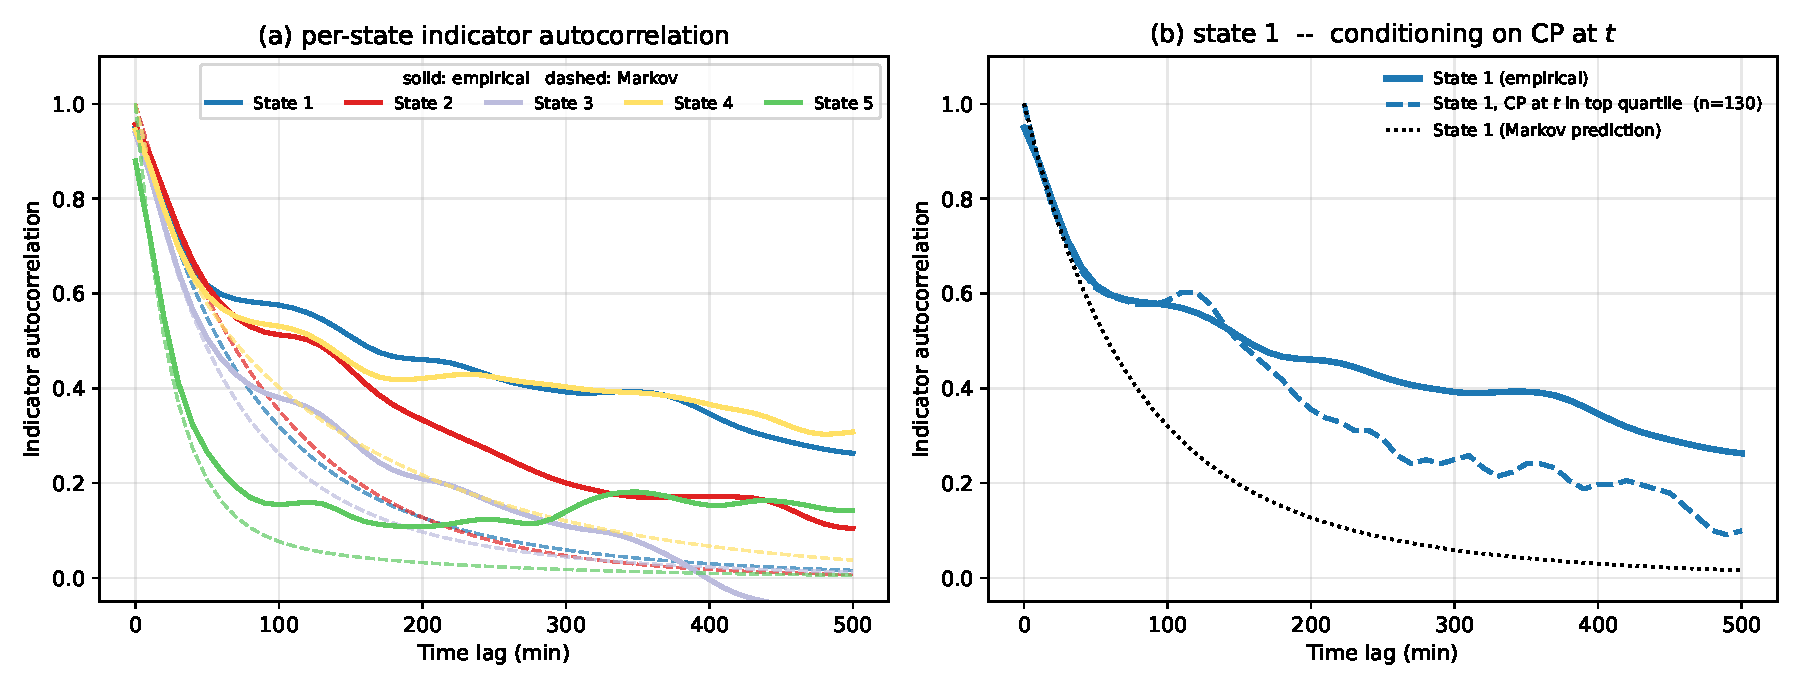
\includegraphics[width=\textwidth]{fig9bis_markovianity_coldpools.pdf}
    \caption{\textbf{Markovianity assessment.} \textbf{(a)}~Per-cluster indicator autocorrelations (solid) and the Markov prediction for the same cluster (dashed, same colour). Clusters~1 and~4 sit visibly above their predictions; the others track theirs closely. \textbf{(b)}~Cluster-1 autocorrelation: empirical (solid blue), Markov prediction (dotted black), and empirical conditioned on the cold-pool intensity $\mathrm{CP}(t)$ at the starting time being above its 75th-percentile threshold $\mathrm{CP}_\star$ (dashed blue). The condition is applied only at the starting time; the trajectory is free thereafter. Cold-pool conditioning closes $\sim$30\% of the empirical--Markov gap at lag 200~min.}
    \label{fig:autocorrelation}
\end{figure}


\section{Conclusion and perspective}\label{sec:conclusion}\label{sec:discussion}
We developed a data-driven framework that treats convective organization dynamically: an encoder maps isentropic mass-flux profiles into a low-dimensional latent space, the latent space is partitioned into discrete convective states, and transitions between states are modelled as a Markov chain. Applied to cloud-resolving squall-line simulations under fixed vertical wind shear, this construction addressed three questions: \emph{(i)} what mass-flux states a given forcing makes accessible; \emph{(ii)} whether transitions between them can be approximated by a Markov chain, and how organized and weakly organized pathways differ; \emph{(iii)} where internal feedbacks introduce effective memory beyond the discrete state.

Convective variability lives on a low-dimensional manifold captured by eight latent dimensions and five discrete states that recover the canonical phases of the convective life cycle. The chain reveals two competing routes through this state space: a direct ascent into sustained deep convection, and a longer drift through weakly organized phases. Clusters~1 and~4 retain residual memory beyond their Markov prediction. Conditioning on cold-pool intensity at the starting time closes roughly $30\%$ of the Cluster~1 gap at a lag of $200$~min.

The framework's distinctive capability is that departures from Markovianity \emph{diagnose} what the discrete partition is missing, identifying the slow internal variables that a closed dynamical description of convection must include.

Within a given forcing, the Markovianity diagnostic can be sharpened by conditioning on richer descriptors of internal state than the domain-integrated cold-pool intensity used here. Because the isentropic mass-flux decomposition retains the downdraft branch of the flow, the representation already exposes the slower time scale on which evaporative downdrafts---and the cold pools they generate---develop relative to the convective updraft; conditioning explicitly on cold-pool age, gust-front strength, and other lifecycle markers would target this development lag directly. Per-cold-pool quantities capture the spatial structure that a scalar index averages out and could be aggregated by cold-pool shape, alignment, or proximity to neighbours; mesoscale moisture pooling, free-tropospheric humidity, and cluster-geometry measures each isolate a further candidate slow variable that the latent state does not currently resolve. Each addition that further closes the empirical-versus-Markov gap identifies another slow variable a memory-aware parameterization must track; the full attribution of the residual Cluster~1 memory is the most direct extension of the present work.


The simulations analysed here span a single shear configuration. The most immediate extension is to repeat the construction across forcing regimes---weak shear (popcorn convection), moderate shear (mixed regimes), strong shear (squall lines)---and compare the resulting transition matrices. The expected shifts are concrete and dynamically interpretable: under stronger shear, the diagonal probabilities $T_{ii}$ of the organized states should increase, the direct pathway from initiation into organized deep convection should dominate over the indirect route through weakly organized phases, and the corresponding eigenmodal time scales should lengthen. Mapping the transition matrix as a function of forcing therefore turns the organization itself into a measurable dynamical observable.



\section{Data and Code Availability}

The simulations analyzed in this study consist of idealized squall-line simulations performed with the System for Atmospheric Modeling (SAM). The dataset spans 27 days of simulation at 2-minute temporal resolution and includes one-dimensional, two-dimensional, and three-dimensional model outputs. The data are available via Globus (link to be provided).

All code used in this study is openly available at: \url{https://github.com/sososquirrel/troposwhere}. The repository includes the implementation of the model as well as the scripts required to reproduce all figures presented in the paper.

\section{Acknowledgments}

We are grateful to Juan Nathanael and Carla Roesch for discussions on Koopman operators, and to Fabrizio Falasca and Matthieu Blanke for recommendations on the dynamical systems literature. We also thank Sara Shamekh, Zhe Feng, Xingchao Chen, Ruby Leung, and the WACCEM project team for valuable discussions throughout the course of this study. We are grateful to Koichi Sakaguchi and Huancui Hu for their time in reviewing the paper and for providing very interesting and constructive feedback.

Portions of the manuscript were rephrased with the assistance of ChatGPT (OpenAI) for language editing, and Claude (Anthropic) assisted with aspects of code development and cleaning. These tools were used solely to improve clarity and software organization; all scientific ideas, analysis, and conclusions were developed by the authors.


This research was supported by the Office of Science of the U.S. Department of Energy (DOE), Biological and Environmental Research (BER), as part of the Regional and Global Modeling and Analysis program area under the Water Cycle and Climate Extremes Modeling (WACCEM) project.

\section{Author Contributions}

S.A. designed the research, performed the simulations, developed the methods and code, and wrote the manuscript. O.P. contributed to the methodological development, contributed to the code, and participated in the analysis and discussions. P.G. contributed to the interpretation of the results and to writing the manuscript.


\printbibliography
\end{document}



\begin{comment}
    \section{Introduction}

Deep convection plays a central role in the transport of mass, energy, and moisture in Earth’s atmosphere, shaping large-scale circulations and extreme weather [add biblio Roca, Feng, Schumacher, Muller]. Yet even under fixed large-scale forcing, convective systems display striking variability: identical environmental conditions can give rise to cloud systems with widely different lifetimes, spatial extents, and degrees of organization [add Houze, Bony, Roca, Leung, Abramian]. This intrinsic variability challenges deterministic descriptions of convection and raises a fundamental question: what diversity of convective systems can arise under a given large-scale forcing?\\

A common strategy for representing this variability is through stochastic parameterizations, in which convective activity is modeled probabilistically rather than deterministically (e.g., Khouider; Majda; Gentine). In these approaches, convective column state is evolving as a Markov chain, with transitions between a small number of idealized convective states and conditioned on large-scale environmental variables. This framework successfully reproduces realistic variability in convective occurrence across space and time. However, because the state space is primarily defined by horizontal location, such models provide limited constraints on the associated vertical redistribution of mass and energy, which governs extreme precipitation (e.g.,Singh, Muller, Bolot).\\

This limitation reflects another aspect in convective dynamics: horizontal organization does not uniquely determine vertical transport. Under comparable large-scale forcing, convective systems can exhibit distinct horizontal structures while producing similar vertical mass-flux profiles, and conversely, geometrically similar systems may differ substantially in their vertical transport (e.g., Greg Elsaesser; Leung; Xingchao). Geometric descriptors such as cloud type or spatial extent are therefore insufficient to characterize the dynamical impact of convection. \\

In this work, we are interested in representing convection defined in terms of its vertical structure. A full-resolution three-dimensional description of convective mass flux leads to an excessively large and noisy state space, obscuring emergence behavior. We look for reducing horizontal spatial resolution to emphasize vertically structured convective configurations within the domain.\\

To do so, we coarse-grain convective mass flux by thermodynamic state using an isentropic analysis (e.g., Pauluis; Mrowiec; Xingchao). Isentropic coordinates provide a thermodynamically consistent framework linking vertical motion to energetic redistribution, yielding a compact, low-dimensional representation while filtering reversible oscillatory motions such as gravity waves. In this isentropic–altitude framework, convection organizes as coherent patterns in mass-flux space rather than as independent evolution at isolated energy levels. This perspective raises two central questions: what is the effective dimensionality of this space, and which vertically structured mass-flux states and transition pathways are accessible under a given large-scale forcing?\\

Representation learning have recently show its power in mapping the high-dimensional space of isentropic mass-flux fields onto a low-dimensional latent space that preserves the dominant structures of convective transport [paper VAE? representation learning]. This approach provides a natural basis for identifying convective states, quantifying transitions among them, and diagnosing the role of stochasticity and internal feedbacks in shaping convective evolution. In this reduced representation, convective evolution appears as trajectories between distinct regions corresponding to dynamically meaningful convective states. \\

In summary, the objective of this study is to characterize the intrinsic variability of deep convection under fixed large-scale forcing through its vertical transport of mass and energy. By representing convection in a reduced space defined by vertically structured mass flux, we seek to identify the dominant modes of convective organization and the pathways through which systems evolve between them. More precisely, we address three questions:

(i) What are the dominant convective mass-flux states accessible under a given large-scale forcing, here characterized by vertical wind shear?
(ii) Can transitions between these states be modeled as a Markov chain, and do transition pathways differ between weak and strongly organized convection?
(iii) To what extent can convective variability be described by memoryless transitions, and how do internal feedbacks, such as cold-pool dynamics, introduce effective memory?\\
\end{comment}